\bookpart{学习}{Learning}
\label{part:pgm-learning}

\BookPartGuide{%
学习把问题从“已知模型怎样计算查询”转为“怎样根据观测确定模型”。数据既可能约束局部条件分布或势函数的数值，也可能提示变量之间的连接；潜变量、缺失字段和观测方式则会使学习过程重新包含推断。

第~\ref{chap:pgm-parameter-learning}章“参数学习”固定图结构，先区分点估计、后验分布与预测分布，再比较完整数据下有向模型、联合无向模型和条件无向模型的归一化方式。潜变量使观测似然需要先汇总未观测状态，EM及其变分、采样近似由此进入参数更新。第~\ref{chap:pgm-structure-learning}章“结构学习”把图本身作为待选对象，用条件独立检验收集局部证据，或用拟合度与复杂度给整张候选图评分，再在庞大的DAG空间中搜索。Markov等价类、CPDAG和忠实性假设说明，纯观测数据通常只能确定部分边和方向；把图解释为因果结构还需要干预或额外机制假设。

两章共同围绕数据能够识别什么展开。参数学习依赖给定的作用域，结构学习则同时选择作用域；缺失变量和错误的观测假设会改变可识别结论。阅读时应区分模型的联合分布、训练目标、推断算法和因果解释，避免把预测用的依赖关系直接表述为因果作用。}

\chapter{参数学习}
\label{chap:pgm-parameter-learning}

到此为止，图的结构和每个局部分布的数值都被当作已知，前八章解决的是“模型给定后怎样做推断”。但这些局部概率（故障率是多少、过热条件下报警有多可能）并不会凭空得到，它们通常要从一批历史设备记录中估计出来。这就是第三部分“学习”的主题，本章先处理其中最基础的\emph{参数学习}：图结构和局部分布的形式（用哪种表、哪种高斯）已经定好，只缺里面的数值参数。设备故障模型$F\to H\to A\leftarrow S$规定了故障、过热、报警和传感器失灵之间的概率分解；要用它预测，还需确定故障率、过热条件概率等局部参数。前面的推断将参数视为已知，本章根据一批设备记录估计参数。

学习的难易首先取决于数据“看得到多少”。所有变量都已记录时，有向模型的参数往往只需数一数各种组合出现多少次，连续情形则退化为局部回归；一旦存在模型主动引入却从未观测的潜在状态，或某些本该记录的字段漏记了，就无法直接计数——此时每更新一次参数，都要先推断这些未观测量的后验分布、用“软计数”代替真实计数，学习于是和前两部分的推断耦合在一起。其次取决于想要什么形式的答案：是给出一个最合适的参数值（点估计），还是给出参数的整个后验分布、把“参数本身有多不确定”也保留下来。这两条选择相互正交、可以组合。后文先说明因子分解与归一化如何决定学习所需的统计量，再讨论潜变量和缺失值怎样引入推断，最后说明参数不确定性如何进入预测。

\section{参数学习的定义}
\label{sec:pgm-parameter-learning-definition}

本节固定学习问题的记号和两种基本准则，后续各节在不同数据可见性下落实它们。设$\mathcal{G}=(V,E)$为固定图，$d=|V|$。记全部节点随机变量为$\bm{W}=(W_1,\ldots,W_d)^\top$，按照数据设计，将其划分为直接记录的字段$\bm{X}$与模型主动设置的潜变量$\bm{Z}$，即在固定排列下$\bm{W}=(\bm{X}^\top,\bm{Z}^\top)^\top$。局部条件分布或势函数由参数向量$\bm{\theta}\in\Theta$控制。可行域$\Theta$包含参数维度以及概率和为$1$、方差为正、配分函数有限等约束。\term{参数学习}（parameter learning）利用记录在这一固定模型族内估计参数点或参数后验。边、潜变量与局部分布族的选择属于模型结构问题，本章把这些选择作为学习的前提。

\term{观测变量}（observed variable）是在当前数据获取设计中直接记录的模型变量，\term{潜变量}（latent variable）则是模型为了表达未观测状态而主动引入的随机量。\term{缺失值}（missing value）指本应记录、却在某条记录中未取得的字段值，它描述数据单元的状态。控制变量分布的参数$\bm{\theta}$则属于估计对象：MLE与MAP将其视为未知的固定优化量，分布估计用先验和后验描述其不确定性。这三个对象分别回答变量如何获取、某个值是否取得，以及分布参数如何估计。

本章用\term{观测完整}表示$\bm{X}$中原定记录的字段均已取得。因此，观测完整且不含潜变量时，每条记录给出全部模型变量；观测完整但含潜变量时，$\bm{X}$没有漏记，$\bm{Z}$仍按模型设定不可见；观测缺失时，$\bm{X}$还要按实际缺失模式拆成已观测部分与缺失部分。潜变量和缺失字段都通过求和或积分从观测似然中消去；缺失字段还涉及值为何未被记录的问题。

以观测完整且不含潜变量的独立记录为例，数据集记为$\mathcal{D}=\{\bm{x}_j\}_{j=1}^n$，其中$x_{j,i}$是第$j$条记录中节点$i$的取值。默认不同记录在给定共同参数后独立同分布，因而$p_{\bm{\theta}}(\mathcal{D})=\prod_jp_{\bm{\theta}}(\bm{x}_j)$。独立性作用于不同完整记录，一条记录内部的节点依赖仍由图描述。同一设备的连续时间观测可能相关，可用第~\ref{chap:pgm-dynamic}章的序列模型或另行处理时间相关性。

局部分布可以使用不同参数块，也可以共享参数。\term{参数共享}（parameter sharing）让多个节点或多条记录使用同一个未知参数，例如同型号传感器共用误报率。同一个共享参数受所有使用位置的局部项约束，估计时应汇总这些项共同优化。逐节点的独立最优值只有满足共享约束时才能构成可行解。

确定了数据记号后，还要规定“什么样的参数算好”。最常用的准则是看这批数据在该参数下出现的可能性有多大：让观测数据的（对数）似然最大的参数称为极大似然估计；若还对参数事先有偏好（先验），就把先验密度也加进去一起最大化，得到极大后验估计。MLE以数据似然比较候选参数，MAP再加入先验密度。令$\ell(\bm{\theta})=\log p_{\bm{\theta}}(\mathcal{D})$。在最优解存在时，两种点估计分别求解
\begin{equation}
  \begin{aligned}
    \widehat{\bm{\theta}}_{\mathrm{ML}}
      &\in\argmax_{\bm{\theta}\in\Theta}\ell(\bm{\theta}),\\
    \widehat{\bm{\theta}}_{\mathrm{MAP}}
      &\in\argmax_{\bm{\theta}\in\Theta}
        \{\ell(\bm{\theta})+\log p(\bm{\theta})\}.
  \end{aligned}
  \label{eq:pgm-parameter-learning-point-objectives}
\end{equation}
似然固定数据后随参数变化，MAP的密度及众数还依赖参数坐标与基准测度。非线性换坐标时，Jacobian进入密度变换。候选集上的最优点可能不唯一；目标也可能只有上确界，因而需要先判断解是否存在（相关统计基础可参考\BookChapterRef{chap:statistical-inference}{卷2《数学准备：概率、因果与决策》的“统计推断”章}）。

MLE和MAP最终都只给出一个参数值，相当于认定“这就是最合适的参数”。但数据有限时，往往有多组参数都与观测相容；要把这种不确定性也保留下来用于预测，就要转而估计参数的后验分布，这就是贝叶斯式的基于分布估计的参数学习。若预测还需要反映多组参数与数据相容的程度，可采用\term{基于分布估计的参数学习}，保留
\begin{equation}
  p(\bm{\theta}\mid\mathcal{D})
  =\frac{p_{\bm{\theta}}(\mathcal{D})p(\bm{\theta})}
  {\int_\Theta p_{\bm{\vartheta}}(\mathcal{D})
    p(\bm{\vartheta})\,\mathrm{d}\bm{\vartheta}},
  \label{eq:pgm-parameter-learning-parameter-posterior}
\end{equation}
分母有限且为正时，先验与数据共同为各参数分配后验权重。这里的随机对象是参数$\bm{\theta}$；固定参数下的变量后验$p_{\bm{\theta}}(\bm{Z}\mid\bm{X})$则用于恢复未观测统计量，两者在学习中承担不同职责。后验均值$\mathbb{E}[\bm{\theta}\mid\mathcal{D}]$在相应平方损失下给出贝叶斯点估计，它是整个参数分布的一项摘要，通常与MLE、MAP不同。

训练准则决定哪些数据分布受到约束。把一条记录分成输入$\bm{x}_j$与输出$\bm{y}_j$后，联合训练与条件训练分别使用
\[
  \begin{aligned}
    \ell_{\mathrm{joint}}(\bm{\theta})
      &=\sum_j\log p_{\bm{\theta}}(\bm{x}_j,\bm{y}_j),\\
    \ell_{\mathrm{cond}}(\bm{\theta})
      &=\sum_j\log p_{\bm{\theta}}(\bm{y}_j\mid\bm{x}_j).
  \end{aligned}
\]
前者同时约束输入和输出的分布；后者把输入当作给定条件，不要求为输入建立概率模型。有向或无向描述因子组织，联合或条件训练描述归一化与拟合的对象，二者可以交叉组合。若两种训练共用某个联合模型的参数，由于
\[
  \log p_{\bm{\theta}}(\bm{x},\bm{y})
  =\log p_{\bm{\theta}}(\bm{y}\mid\bm{x})
   +\log p_{\bm{\theta}}(\bm{x}),
\]
两种目标一般会选择不同的参数。第~\ref{sec:pgm-parameter-learning-complete}至\ref{sec:pgm-parameter-learning-incomplete}节先沿数据可见性轴讨论MLE与MAP点估计，第~\ref{sec:pgm-parameter-learning-bayesian}节再沿分布估计轴说明怎样保留$p(\bm{\theta}\mid\mathcal{D})$；各种数据可见性设定都可以采用点估计或分布估计\scite{pgm-koller2009}

\section{观测完整且不含潜变量的参数学习}
\label{sec:pgm-parameter-learning-complete}

本节处理所有模型变量都被完整观测、没有潜变量和漏记的情形。三类图模型的学习难度并不相同，差别来自归一化方式：有向图的每个局部条件分布各自归一化，所以学习可以拆成彼此独立的小问题，常常退化为计数；联合无向图的势函数乘积靠全局配分函数一起归一化，改一个势会牵动全局，学习时必须做模型推断；条件无向图则对每个给定输入只在标签上归一化。本节比较三类图模型的MLE与MAP点估计。

\subsection{有向图模型}
\label{sec:pgm-parameter-learning-directed}

完整数据下，有向模型的参数学习可拆成若干独立的局部条件分布估计，因为联合似然天然分解为只含一组局部参数的条件分布之积。取对数后乘积变求和，再对样本求和，就得到
\begin{equation}
  \begin{aligned}
    \ell(\bm{\theta})
      &=\sum_{j=1}^n\sum_{i=1}^d
        \log p_{\bm{\theta}_i}
        (x_{j,i}\mid\bm{x}_{j,\operatorname{pa}(i)})\\
      &=\sum_{i=1}^d\ell_i(\bm{\theta}_i).
  \end{aligned}
  \label{eq:pgm-parameter-learning-dag-likelihood}
\end{equation}
若不同节点的参数块没有共享约束，且$\Theta=\prod_i\Theta_i$，最大化每个$\ell_i$就能最大化总似然。目标可加、参数域可分使这些局部最优点组合成全局最优点。本节父节点均有实测值，因此可以直接拟合子节点的条件分布，父节点彼此的相关性仍由其他局部项描述。

对离散节点，\term{条件概率表}（conditional probability table, CPT）逐行列出每种父节点配置下的子节点分布。设$X_i$有$r_i$个状态，以$a$索引其父节点的取值配置。用$\theta_{i,a,k}$表示该配置下$X_i=k$的条件概率，约束为$\theta_{i,a,k}\geq0$及$\sum_k\theta_{i,a,k}=1$。把相同局部事件的出现次数归并，得到
\begin{equation}
  \begin{aligned}
    N_{i,a,k}
      &=\sum_{j=1}^n
        \mathbf{1}\{x_{j,i}=k,\,
          \bm{x}_{j,\operatorname{pa}(i)}=a\},\\
    N_{i,a}&=\sum_{k=1}^{r_i}N_{i,a,k},\qquad
    \ell_i=\sum_a\sum_{k=1}^{r_i}
      N_{i,a,k}\log\theta_{i,a,k}.
  \end{aligned}
  \label{eq:pgm-parameter-learning-counts}
\end{equation}
于是离散有向模型的MLE朴素得惊人：每个条件概率就等于“相应父配置下，子节点取某值的次数除以该父配置出现的总次数”，即按经验频率填表。关于参数的似然仅通过这些计数依赖记录，故它们构成当前局部模型的\term{充分统计量}（sufficient statistic）——有了这些计数，逐条数据的其他细节对估计参数不再提供额外信息。根节点只有一个空的父配置，其计数就是通常的类别频数。

固定一行$a$，在内部解上加入约束项$\lambda(1-\sum_k\theta_{i,a,k})$。对$\theta_{i,a,k}$求导得到$N_{i,a,k}/\theta_{i,a,k}=\lambda$，再对$k$求和得到$\lambda=N_{i,a}$。允许零计数对应边界解，并约定$0\log0=0$，可得
\begin{equation}
  \widehat{\theta}_{i,a,k,\mathrm{ML}}
    =\frac{N_{i,a,k}}{N_{i,a}},\qquad N_{i,a}>0.
  \label{eq:pgm-parameter-learning-cpt-mle}
\end{equation}
$N_{i,a}=0$时没有记录使用该父配置，整行概率在似然中都不受约束，此时需要先验或额外数据来确定它。若可行域要求概率严格为正，含零计数的行可能只能趋近边界上确界，内部最优点未必存在。

纯经验频率有个问题：某种父配置若一次都没出现（$N_{i,a}=0$），对应那行概率数据完全没给出信息；即使出现了，次数很少时估计也极不稳。一个自然的补救是先往每个格子里放一些“虚拟的先验计数”，把先验知识和数据计数合在一起。用逐行独立的\term{Dirichlet先验}（Dirichlet prior）为整行概率分配先验权重，可以将已有知识加入局部估计：
\[
  p(\bm{\theta}_{i,a})
  \propto\prod_{k=1}^{r_i}
    \theta_{i,a,k}^{\alpha_{i,a,k}-1},
  \qquad \alpha_{i,a,k}>0.
\]
把对数先验加入局部对数似然，仍可逐行求MAP。记$\alpha_{i,a,0}=\sum_k\alpha_{i,a,k}$；当所有$\alpha_{i,a,k}+N_{i,a,k}>1$时，内部众数为
\begin{equation}
  \widehat{\theta}_{i,a,k,\mathrm{MAP}}
    =\frac{N_{i,a,k}+\alpha_{i,a,k}-1}
            {N_{i,a}+\alpha_{i,a,0}-r_i}.
  \label{eq:pgm-parameter-learning-cpt-map}
\end{equation}
上述条件保证众数位于内部；其余情形应根据边界密度判断众数及唯一性。均匀Dirichlet先验下，内部MAP与MLE相同。“加一平滑”来自该先验的后验均值，第~\ref{sec:pgm-parameter-learning-conjugacy}节将给出完整后验及其摘要。

以下用人工构造的设备记录贯穿计数、EM与参数后验计算。样本频数描述本批教学记录，前章的模型概率描述生成分布，二者承担不同角色。表~\ref{tab:pgm-parameter-learning-device-counts}列出$20$条完整记录在$(F,H)$上的边缘计数；$A,S$的记录不参与这里展示的两个局部参数块。

\begin{table}[htbp]
  \centering
  \begin{tabular}{lrrr}
    \toprule
    故障状态 & $H=1$ & $H=0$ & 合计\\
    \midrule
    $F=1$ & $4$ & $1$ & $5$\\
    $F=0$ & $2$ & $13$ & $15$\\
    \midrule
    合计 & $6$ & $14$ & $20$\\
    \bottomrule
  \end{tabular}
  \caption{人工构造的局部计数，所有观测字段均无缺失。根节点故障率使用总记录数为分母，条件过热率使用相应故障行的合计为分母。}
  \label{tab:pgm-parameter-learning-device-counts}
\end{table}

由计数可得$\widehat p(F=1)=5/20=0.25$，而$\widehat p(H=1\mid F=1)=4/5=0.8$、$\widehat p(H=1\mid F=0)=2/15$。若只对故障率$\pi=p(F=1)$使用$\operatorname{Beta}(2,2)$先验，即二元Dirichlet先验，则MLE为$1/4$，MAP为$6/22=3/11\approx0.2727$。MAP将先验加入点估计目标。第~\ref{sec:pgm-parameter-learning-conjugacy}节将用同一组计数计算参数后验及后验均值。

连续节点也能利用局部分解。对线性高斯条件分布，设父节点数为$m_i$，将截距与父节点组成$\bm{u}_{j,i}=(1,\bm{x}_{j,\operatorname{pa}(i)}^\top)^\top$，并令
\[
  X_i\mid\bm{X}_{\operatorname{pa}(i)}
  \sim\mathcal{N}(\bm{\beta}_i^\top\bm{u}_i,\sigma_i^2).
\]
去掉与参数无关的常数，局部负对数似然为
\[
  -\ell_i
  =\frac{n}{2}\log\sigma_i^2+
    \frac{1}{2\sigma_i^2}
      \sum_{j=1}^n(x_{j,i}-\bm{\beta}_i^\top\bm{u}_{j,i})^2.
\]
将$\bm{u}_{j,i}^\top$按样本顺序堆叠为设计矩阵$\bm{U}_i$，它有$n$行、$m_i+1$列。响应向量为$\bm{y}_i=(x_{1,i},\ldots,x_{n,i})^\top$。固定正方差，对回归系数求导得到正规方程；在$\bm{U}_i$列满秩且残差平方和为正时，
\begin{equation}
  \begin{aligned}
    \widehat{\bm{\beta}}_i
      &=(\bm{U}_i^\top\bm{U}_i)^{-1}\bm{U}_i^\top\bm{y}_i,\\
    \widehat{\sigma}_i^2
      &=\frac{1}{n}
        \lVert\bm{y}_i-\bm{U}_i\widehat{\bm{\beta}}_i\rVert_2^2.
  \end{aligned}
  \label{eq:pgm-parameter-learning-gaussian-mle}
\end{equation}
这里估计的是似然最优方差，分母为$n$；无偏残差方差估计则使用$n-m_i-1$。秩亏会使回归系数不唯一，零残差与任意接近$0$的方差会使似然无界。实现时可用设计矩阵的QR分解求解回归系数，避免显式逆矩阵。完整有向模型因而将学习分解为局部计数或回归，数据覆盖、设计秩及参数共享决定局部解能否组成所需估计。

\subsection{联合无向图}
\label{sec:pgm-parameter-learning-undirected}

有向模型的局部归一化使学习成为数数，无向模型则要麻烦得多：势函数本身未归一化，它们要靠一个对所有变量求和的全局配分函数$Z$归一化，而$Z$依赖全部参数。这意味着改一个势的参数，所有配置的归一化概率都会随之改变，似然不再能拆成彼此独立的局部项。联合无向模型通过全局配分函数归一化局部势的乘积。考虑固定支持集$\mathcal{X}$上的正指数族模型
\begin{equation}
  \begin{aligned}
    p_{\bm{\theta}}(\bm{x})
      &=h(\bm{x})
        \exp\{\bm{\theta}^\top\bm{T}(\bm{x})-A(\bm{\theta})\},\\
    A(\bm{\theta})&=\log Z(\bm{\theta}),\\
    Z(\bm{\theta})
      &=\int_{\mathcal{X}}h(\bm{x})
        e^{\bm{\theta}^\top\bm{T}(\bm{x})}\,\mathrm{d}\mu(\bm{x}).
  \end{aligned}
  \label{eq:pgm-parameter-learning-exponential-model}
\end{equation}
$\bm{T}$收集团上的充分统计量，$h$是与参数无关的基准因子，$\mu$在离散情形取计数测度，在连续情形取相应基准测度。要求$0<Z(\bm{\theta})<\infty$。令$\overline{\bm{T}}=n^{-1}\sum_j\bm{T}(\bm{x}_j)$，平均对数似然中与参数有关的部分为$\bm{\theta}^\top\overline{\bm{T}}-A(\bm{\theta})$。

参数改变一个局部势时，也会改变全局归一化常数。在可交换微分与积分的条件下，对数归一化项的导数为
\begin{equation}
  \begin{aligned}
    \nabla_{\bm{\theta}} A(\bm{\theta})
      &=\frac{1}{Z(\bm{\theta})}
        \int h(\bm{x})e^{\bm{\theta}^\top\bm{T}(\bm{x})}
             \bm{T}(\bm{x})\,\mathrm{d}\mu(\bm{x})\\
      &=\mathbb{E}_{p_{\bm{\theta}}}[\bm{T}(\bm{X})],\\
    \frac{1}{n}\nabla_{\bm{\theta}}\ell(\bm{\theta})
      &=\overline{\bm{T}}
        -\mathbb{E}_{p_{\bm{\theta}}}[\bm{T}(\bm{X})].
  \end{aligned}
  \label{eq:pgm-parameter-learning-moment-gradient}
\end{equation}
有限离散支持下可逐项求导；连续情形可由参数邻域内的可积支配函数等正则条件保证交换。梯度比较了数据实际呈现的统计量与模型预期的统计量：沿梯度上升时，经验统计量大于模型期望的坐标增加，小于模型期望的坐标减小。梯度的含义非常直观：它比较的是“数据里实际观察到的统计量平均$\overline{\bm T}$”与“模型在当前参数下预期会产生的统计量$\mathbb E_{\bm\theta}\bm T$”。数据中出现得比模型预期更频繁的模式（梯度为正）就增强对应参数，出现得更少的模式（梯度为负）就减弱；当两者完全吻合时梯度为零，正是MLE的驻点条件。最优内部点满足矩匹配，但数据矩落在可实现矩集合的边界时，有限参数MLE可能不存在。

再求一次导数，得到$\nabla^2A=\operatorname{Cov}_{p_{\bm{\theta}}}[\bm{T}(\bm{X})]$，所以线性自然参数下的对数似然是凹函数。冗余统计量可使协方差奇异，因而仍可能有多个参数最优点。凹性建立在线性自然参数化上；使用非线性网络势时，应重新分析关于网络参数的曲率。指数族与矩匹配的关系可回顾第~\ref{chap:pgm-variational}章\scite{pgm-wainwright2008}

一个只有两个节点的例子可以直接核验梯度。设$X_1,X_2\in\{-1,1\}$，$p_\theta(x_1,x_2)\propto e^{\theta x_1x_2}$。同号和异号各有两个配置，因此$Z(\theta)=2e^\theta+2e^{-\theta}=4\cosh\theta$，模型期望为$\mathbb{E}_\theta[X_1X_2]=\tanh\theta$。若$10$条记录中有$8$条同号、$2$条异号，则经验统计量为$0.6$，平均似然梯度为$0.6-\tanh\theta$。令它为零，得到$\widehat\theta=\operatorname{arctanh}(0.6)=\log2$；代回模型，同号概率$e^\theta/(e^\theta+e^{-\theta})=0.8$，恰好匹配记录。

四配置例可以枚举所有模型状态。这个梯度里的模型期望$\mathbb E_{\bm\theta}\bm T$正是第~\ref{chap:pgm-elimination}章起讨论的推断问题——它要在当前参数下对全部配置求和；图一大就和精确推断一样困难。这暴露出无向模型学习的核心特征：\emph{学习的内层嵌套着推断}。大图中的模型期望则可能需要高维求和，即使梯度计算没有显式输出$Z$，求期望仍是推断任务。降低成本有两条路线：一是老老实实用前两章的（精确或近似）推断算准这个期望，二是干脆换一个不含全局归一化、更容易优化的替代学习准则。

第一条路线保留式~\eqref{eq:pgm-parameter-learning-moment-gradient}的模型期望。用MCMC产生近似服从$p_{\bm{\theta}}$的样本，再用样本均值估计模型期望；链混合不足带来偏差，样本相关性降低有效样本量。也可以通过变分推断取得近似边缘分布，计算所需的局部统计量。若使用的是某个近似对数配分函数$\widetilde A$的梯度，实际优化的便是$\bm{\theta}^\top\overline{\bm{T}}-\widetilde A(\bm{\theta})$。近似边缘所给的更新方向，需要通过相应近似目标或误差分析来解释。若这些边缘并非由同一近似配分函数的导数产生，更新可能无法对应一个固定标量目标，精确似然的单调性也需另行判断。

另一条路线主动更换准则。\term{伪似然}（pseudolikelihood）把每个节点在其余节点已知时的条件概率相乘，用一组容易归一化的预测问题替代联合密度拟合。沿用第~\ref{sec:pgm-undirected-local}节的邻居集合$N(i)$，正无向模型满足
\begin{equation}
  \ell_{\mathrm{PL}}(\bm{\theta})
  =\sum_{j=1}^n\sum_{i=1}^d
    \log p_{\bm{\theta}}
      (x_{j,i}\mid\bm{x}_{j,N(i)}).
  \label{eq:pgm-parameter-learning-pseudolikelihood}
\end{equation}
固定邻居后，不含$i$的势函数与全局$Z$一起约掉，只需对$X_i$归一化。二值节点只涉及两个候选值，因此常比全局求和容易。这些条件项组成伪似然训练准则，其数值衡量局部条件预测；联合预测评价仍需原模型的归一化联合概率。

\term{复合似然}（composite likelihood）进一步组合若干低维边缘或条件似然，其对数形式是这些局部对数似然按固定非负权重相加，伪似然是其中一个特例。选择可计算的条件块可以避开全局归一化；若选择的边缘块本身仍难以求出，则并没有消除推断困难。在模型正确、所用局部项能够识别参数且满足通常的估计正则条件时，这类估计可以一致，但有限样本解和统计效率一般不同于MLE。相应标准误需采用适合复合准则的方差估计\scite{pgm-parameter-learning-varin2011}

若模型只给出非归一化密度，还可以把估计转化为区分数据与已知噪声的分类任务。\term{噪声对比估计}（noise-contrastive estimation, NCE）选择已知且覆盖数据支持的噪声密度$p_{\mathrm{N}}$，对每个数据样本抽取$\nu$个噪声样本，这里$\nu$为正整数。在合并后的样本中，$D=1$表示来自数据，$D=0$表示来自噪声，来源先验为$P(D=1)=1/(1+\nu)$、$P(D=0)=\nu/(1+\nu)$。若真实数据密度为$p_*$，则贝叶斯公式给出
\[
  \begin{aligned}
    P(D=1\mid\bm{x})
      &=\frac{p_*(\bm{x})P(D=1)}
        {p_*(\bm{x})P(D=1)+p_{\mathrm{N}}(\bm{x})P(D=0)}\\
      &=\frac{p_*(\bm{x})}
        {p_*(\bm{x})+\nu p_{\mathrm{N}}(\bm{x})}.
  \end{aligned}
\]
因此，分母中的$\nu$来自两类样本的数量比例。

用$\widetilde p_{\bm{\theta},c}(\bm{x})=\exp\{f_{\bm{\theta}}(\bm{x})+c\}$拟合数据密度，并把负对数归一化常数作为额外标量$c$学习，就得到来源分类概率模型
\[
  a_{\bm{\theta},c}(\bm{x})
  =\frac{\widetilde p_{\bm{\theta},c}(\bm{x})}
         {\widetilde p_{\bm{\theta},c}(\bm{x})
                +\nu p_{\mathrm{N}}(\bm{x})}.
\]
$a_{\bm{\theta},c}(\bm{x})$是给定样本后“它来自数据”的概率，$\widetilde p_{\bm{\theta},c}(\bm{x})$则是待学习的数据密度形式；优化过程中后者未必已经归一化。

最大化二分类对数似然
\[
  \begin{aligned}
    J_{\mathrm{NCE}}
      &=\sum_{j=1}^n\log a_{\bm{\theta},c}(\bm{x}_j)\\
      &\quad+\sum_{l=1}^{\nu n}
        \log\{1-a_{\bm{\theta},c}(\bm{y}_l)\},
        \qquad \bm{y}_l\sim p_{\mathrm{N}},
  \end{aligned}
\]
无需在每一步计算$Z$。在正确设定和可识别等条件下，NCE可以一致估计密度；有限噪声样本下优化的是来源分类似然，与MLE的数据似然不同。噪声覆盖不足或分类任务过易会影响参数信息。来源标签$D$是估计构造的辅助变量，原图中的预测任务仍由学得的数据模型承担\scite{pgm-parameter-learning-gutmann2012}

对连续、光滑且正的密度，还有另一种消去归一化常数的方法。\term{分数匹配}（score matching）以数据空间中的对数密度梯度$\bm{s}_{\bm{\theta}}(\bm{x})=\nabla_{\bm{x}}\log p_{\bm{\theta}}(\bm{x})$为匹配对象；对参数求导的似然得分则是另一种导数。由于$\log Z(\bm{\theta})$不依赖$\bm{x}$，它在这里消失。若真实密度$p_*$及模型满足可积性条件，且分部积分的边界项为零，则
\begin{equation}
  \begin{aligned}
    J_{\mathrm{SM}}(\bm{\theta})
      &=\frac12\mathbb{E}_{p_*}
          \lVert\bm{s}_{\bm{\theta}}-\nabla_{\bm{x}}\log p_*\rVert_2^2\\
      &=\mathbb{E}_{p_*}\!\left[
          \frac12\lVert\bm{s}_{\bm{\theta}}\rVert_2^2+
          \nabla_{\bm{x}}\!\cdot\bm{s}_{\bm{\theta}}
        \right]+C.
  \end{aligned}
  \label{eq:pgm-parameter-learning-score-matching}
\end{equation}
$C$与模型参数无关。关键一步是分部积分：
\[
  -\int\bm{s}_{\bm{\theta}}^\top\nabla p_*\,\mathrm{d}\bm{x}
  =\int p_*\nabla\cdot\bm{s}_{\bm{\theta}}\,\mathrm{d}\bm{x}.
\]
因此未知的真实分数从可优化部分消失，可以用训练样本均值替代期望。标准形式的适用范围是可微且满足边界条件的连续密度，离散变量和受限支持需另作构造。所优化的量是两个数据分数的平方差\scite{pgm-parameter-learning-hyvarinen2005}

还可以用短链降低模型期望的计算成本。\term{对比散度}（contrastive divergence, CD）通常从训练样本启动以$p_{\bm{\theta}}$为平稳分布的Markov链，运行$k$步，以终点统计量替代模型期望。若经验分布为$\widehat p$、转移核为$K_{\bm{\theta}}$，则其期望更新方向为
\[
  \bm{g}_{\mathrm{CD},k}
    =\mathbb{E}_{\widehat p}[\bm{T}]
      -\mathbb{E}_{\widehat pK_{\bm{\theta}}^k}[\bm{T}].
\]
有限$k$时，$\widehat pK_{\bm{\theta}}^k$通常不同于$p_{\bm{\theta}}$，因此增加平行链数虽能消除Monte Carlo波动，有限步终点分布与模型分布的差异仍可留下偏差。虽然名称来自两个KL散度之差，但链终点分布也依赖参数；通常更新省略了这部分导数，相应方向一般与该KL差的精确梯度不同。二值受限玻尔兹曼机已有更新方向无法对应一般标量目标的反例；特殊转移核的对应关系需限定其构造\scite{pgm-parameter-learning-sutskever2010}

\term{持久链}（persistent chain）在下一次参数更新时沿用上次的链状态，避免每次都从数据重新启动。它试图在模型缓慢变化时持续跟踪模型分布，但固定的少量转移并不保证链已达到新参数下的平稳状态。充分混合的MCMC与有限步持久链使用同一个模型期望公式，区别在于后者依赖跨迭代跟踪的近似；CD还固定采用数据初始化。它们与伪似然、NCE和分数匹配的区别，则在于后几种方法明确改变了学习准则。比较这些方法时，可分别报告期望近似的误差、实际训练准则和计算预算\scite{goodfellow2016}

\subsection{条件无向图}
\label{sec:pgm-parameter-learning-conditional}

很多任务只关心“给定输入预测输出”（如图像标注、序列标注），并不需要对输入本身建模。此时可以把输入当作固定条件，归一化只在可能的标签上进行——这既省去了对输入建模，也让每个样本有自己的归一化项。若目标是根据已经给出的测量$\bm{x}$预测一组标签$\bm{y}$，就可以只归一化标签空间。\term{条件随机场}（conditional random field, CRF）通过局部特征组织一个条件联合分布，让多个标签在给定输入以后仍能相互依赖。在线性参数化下写为
\begin{equation}
  \begin{aligned}
    p_{\bm{\theta}}(\bm{y}\mid\bm{x})
      &=\frac{\exp\{\bm{\theta}^\top\bm{f}(\bm{x},\bm{y})\}}
              {Z_{\bm{\theta}}(\bm{x})},\\
    Z_{\bm{\theta}}(\bm{x})
      &=\sum_{\bm{y}'}
         \exp\{\bm{\theta}^\top\bm{f}(\bm{x},\bm{y}')\}.
  \end{aligned}
  \label{eq:pgm-parameter-learning-crf}
\end{equation}
特征$\bm{f}$通常是各团特征的和，可以依赖整个已知输入；图主要限制标签之间的相互作用。每个输入对应自己的条件配分函数，训练目标因而逐记录计算归一化项。

对完整标签训练集$\{(\bm{x}_j,\bm{y}_j)\}_{j=1}^n$，以$\lambda\geq0$控制二次正则化，目标及梯度为
\begin{equation}
  \begin{aligned}
    J(\bm{\theta})
      &=\sum_{j=1}^n
        \left[\bm{\theta}^\top\bm{f}(\bm{x}_j,\bm{y}_j)
                    -\log Z_{\bm{\theta}}(\bm{x}_j)\right]\\
      &\quad-\frac{\lambda}{2}\lVert\bm{\theta}\rVert_2^2,\\
    \nabla_{\bm{\theta}}J
      &=\sum_{j=1}^n
        \left[\bm{f}(\bm{x}_j,\bm{y}_j)
          -\mathbb{E}_{p_{\bm{\theta}}(\bm{Y}\mid\bm{x}_j)}
             \bm{f}(\bm{x}_j,\bm{Y})\right]\\
      &\quad-\lambda\bm{\theta}.
  \end{aligned}
  \label{eq:pgm-parameter-learning-crf-gradient}
\end{equation}
推导与无向联合模型相同，只是每次都固定输入再求和。梯度比较给定输入下已观测标签的特征，与模型对所有候选标签的平均特征。$\lambda>0$时，正则项也可解释为各参数服从方差$\lambda^{-1}$的零均值高斯先验所产生的MAP项。

例如，只有一个二元标签、一个标量特征$f(x,y)=yx$时，$p_\theta(Y=1\mid x)=\operatorname{sigmoid}(\theta x)$。单条记录$(x,y)=(2,1)$在$\theta=0$处贡献梯度$2-2\times0.5=1$，推动正类概率上升。多个相互依赖的标签使这种期望计算变复杂：线性链可以通过前向后向递推计算局部边缘，一般图则可能需要近似推断。固定特征的线性CRF具有凹的条件对数似然，但无正则化时仍可能因可分离等情形没有有限最优解；神经特征参与学习时也不再一般地凹。第~\ref{chap:pgm-energy-models}章将展开具体CRF结构及其计算。

\section{观测完整但含潜变量的参数学习}
\label{sec:pgm-parameter-learning-latent}

完整数据下有向模型靠数数就能学，但现实中常常有一些变量根本观察不到——它们是模型为解释数据而主动引入的潜变量（如混合模型里“样本属于哪个类”的隐类别）。这时真实计数无从得知：我们不知道每条记录对应哪个隐状态。自然的替代是用该事件在当前参数、当前观测下的\emph{后验概率}充当“软计数”，而这每一步都要调用推断。本节的数据字段$\bm{X}$全部取得，模型中的潜变量$\bm{Z}$仍不可见。要统计包含$\bm{Z}$的局部事件，就需计算这些事件在已知记录下的后验概率；连续模型则需相应的条件矩。以下先建立观测数据似然，再讨论精确EM、GEM、近似E步和摊销推断如何提供这些统计量并更新参数。主要输出仍是MLE或MAP参数点。

\subsection{观测数据似然}
\label{sec:pgm-parameter-learning-marginal-likelihood}

当前记录可能由潜变量的多种取值产生。将这些取值的联合概率加总，才能得到该记录在候选参数下的概率：
\begin{equation}
  \ell(\bm{\theta})
    =\sum_{j=1}^n\log p_{\bm{\theta}}(\bm{x}_j)
    =\sum_{j=1}^n
       \log\int p_{\bm{\theta}}(\bm{x}_j,\bm{z}_j)
                         \,\mathrm{d}\bm{z}_j.
  \label{eq:pgm-parameter-learning-observed-likelihood}
\end{equation}
离散变量把积分换成求和。这里的\term{边缘似然}（marginal likelihood）是消去潜变量之后、仍作为$\bm{\theta}$函数的观测似然；它不同于式~\eqref{eq:pgm-parameter-learning-parameter-posterior}分母中进一步积分参数所得的模型证据。前者用于本章的参数优化，后者常用于模型比较。

每条记录的概率包含潜变量积分，因而对数似然通常无法按完整配置的真实计数直接分解。在微分与积分可交换、观测密度为正时，
\begin{equation}
  \begin{aligned}
    \nabla_{\bm{\theta}}\log p_{\bm{\theta}}(\bm{x}_j)
      &=\frac{\int\nabla_{\bm{\theta}}
          p_{\bm{\theta}}(\bm{x}_j,\bm{z}_j)
                  \,\mathrm{d}\bm{z}_j}
             {p_{\bm{\theta}}(\bm{x}_j)}\\
      &=\mathbb{E}_{p_{\bm{\theta}}(\bm{Z}_j\mid\bm{x}_j)}
          [\nabla_{\bm{\theta}}
            \log p_{\bm{\theta}}(\bm{x}_j,\bm{Z}_j)].
  \end{aligned}
  \label{eq:pgm-parameter-learning-fisher-identity}
\end{equation}
第二个等号使用$\nabla p=p\nabla\log p$，再将联合密度除以观测密度识别为后验。这说明直接梯度优化同样需要当前参数下的后验推断。对离散CPT，原来的事件指示量要换成“该事件在当前观测下发生的后验概率”。这些后验概率随参数变化，更新参数后需要重新计算。

沿用表~\ref{tab:pgm-parameter-learning-device-counts}的过热总数，考虑另一种模型：数据字段只有$H$，故障状态$F$被主动设置为潜变量；$A,S$在这次教学计算中不进入模型。为了只研究一个未知量，把过热条件概率固定为另行给定的校准值$p(H=1\mid F=1)=0.8$和$p(H=1\mid F=0)=0.1$，仅学习$\pi=p(F=1)$。于是
\[
  p_\pi(H=1)=0.8\pi+0.1(1-\pi)=0.1+0.7\pi.
\]
$20$条记录中$6$条过热、$14$条不过热，观测对数似然为
\begin{equation}
  \ell(\pi)=6\log(0.1+0.7\pi)
             +14\log(0.9-0.7\pi),\qquad 0\leq\pi\leq1.
  \label{eq:pgm-parameter-learning-device-observed}
\end{equation}
它在$p_\pi(H=1)=6/20$处最大，故$\widehat\pi_{\mathrm{ML}}=2/7$。这个一维例子可以直接解出，适合用来检查EM；更复杂图中的边缘似然通常不能这样化简。若把两项过热条件概率也设为未知，单一的过热频率便不足以识别三个参数，困难就不只是如何优化了。

\subsection{精确EM}
\label{sec:pgm-parameter-learning-em}

面对潜变量，一个朴素想法是先“猜”每个潜变量的取值（比如取后验概率最大的那个），再当作完整数据去数数更新参数。但这样硬猜会把不确定的推断结果当成既成事实，丢掉其他可能取值的贡献，而且猜错会自我强化。EM的做法更稳妥：不把潜变量钉死在某个值上，而是按当前参数算出它取各值的后验概率，用这些概率作为软权重去计算“期望计数”，再据此更新参数；然后用新参数重新算后验，如此交替。式~\eqref{eq:pgm-parameter-learning-fisher-identity}把未知状态换成后验平均。将观测量与潜变量合在一起，得到\term{完全数据}（complete data）$(\bm{X},\bm{Z})$。这个计算对象允许我们描述完整配置下的似然，实际记录仍只有$\bm{X}$。若给定完全数据后容易求出最优参数，我们可以进一步利用这一结构：在当前参数下算出潜变量的后验统计量，再把它们固定下来更新参数。\term{期望最大化算法}（expectation-maximization algorithm, EM）正是这样交替进行推断与优化；E步保留潜变量各取值的后验权重，M步利用这些权重形成的期望统计量。

现在要把这种交替更新与原来的观测似然联系起来。如果先把每个未知状态猜成一个值，猜错的记录就会被当作确定事实。EM保留各个潜在配置的后验权重，并用这些权重构造一个更容易优化的辅助目标。这个目标须满足两个条件：对所有候选参数都不超过观测对数似然，在当前参数处又恰好等于观测对数似然。这样，提高辅助目标才能保证原似然不下降。为构造这一目标，对每条记录引入潜变量分布$q_j(\bm{z}_j)$。先取它在相应联合密度为正的支持上为正，并假设下式期望与熵有限。利用$\log$的凹性和Jensen不等式，
\begin{equation}
  \begin{aligned}
    \log p_{\bm{\theta}}(\bm{x}_j)
      &=\log\mathbb{E}_{q_j}
        \left[\frac{p_{\bm{\theta}}(\bm{x}_j,\bm{Z}_j)}
                    {q_j(\bm{Z}_j)}\right]\\
      &\geq
        \mathbb{E}_{q_j}\log p_{\bm{\theta}}
             (\bm{x}_j,\bm{Z}_j)+\mathcal{H}(q_j),
  \end{aligned}
  \label{eq:pgm-parameter-learning-jensen}
\end{equation}
其中$\mathcal{H}(q_j)=-\mathbb{E}_{q_j}\log q_j$，连续情形为微分熵。每条记录的右侧就是式~\eqref{eq:pgm-variational-elbo}中的$\mathcal{L}(q_j)$；这里只是显式恢复待学习的模型参数。把各条记录相加，记下界为$\mathcal{F}(q,\bm{\theta})$。

更精确的关系是
\begin{equation}
  \begin{aligned}
    \mathcal{F}(q,\bm{\theta})
      &=\sum_j\{\mathbb{E}_{q_j}
          \log p_{\bm{\theta}}(\bm{x}_j,\bm{Z}_j)
                      +\mathcal{H}(q_j)\},\\
    \ell(\bm{\theta})
      &=\mathcal{F}(q,\bm{\theta})
        +\sum_j\operatorname{KL}
          \bigl(q_j\,\|\,p_{\bm{\theta}}(\bm{Z}_j\mid\bm{x}_j)\bigr).
  \end{aligned}
  \label{eq:pgm-parameter-learning-elbo-identity}
\end{equation}
第二式直接由后验密度的定义代入KL散度得到；只要$q_j$对后验绝对连续且各项有限，它也适用于$q_j$仅覆盖部分后验支持的情况。这就是本章使用的\term{证据下界}（evidence lower bound, ELBO）：它的下界对象是当前参数下的观测对数似然。KL散度非负，并且在$q_j$等于真实后验时为零，因此这个下界可以在当前参数处与似然相等。

固定第$t$次参数$\bm{\theta}^{(t)}$，E步取
\[
  q_j^{(t)}(\bm{z}_j)
    =p_{\bm{\theta}^{(t)}}(\bm{z}_j\mid\bm{x}_j).
\]
E步因而在当前参数处把下界抬到似然本身。M步随后固定这些分布，只改变模型参数；后验熵此时是常数，所以只需最大化完全数据对数似然的后验期望。定义
\begin{equation}
  \begin{aligned}
    Q(\bm{\theta}\mid\bm{\theta}^{(t)})
      &=\sum_j\mathbb{E}_{q_j^{(t)}}
          \log p_{\bm{\theta}}(\bm{x}_j,\bm{Z}_j),\\
    \bm{\theta}^{(t+1)}
      &\in\argmax_{\bm{\theta}\in\Theta}
         Q(\bm{\theta}\mid\bm{\theta}^{(t)}).
  \end{aligned}
  \label{eq:pgm-parameter-learning-em-update}
\end{equation}
熵在M步中不依赖新参数，所以最大化$Q$等价于最大化固定$q^{(t)}$的下界。旧参数决定积分分布，新参数进入完全数据的对数密度。M步固定前者，才能优化同一个下界；随后新的E步再更新积分分布。

\begin{theorem}[EM的观测似然单调性]
  \label{thm:pgm-parameter-learning-em-monotonicity}
  设$\bm{x}_1,\ldots,\bm{x}_n$为固定观测，$\bm{Z}_j$为第$j$条记录的潜变量。对每个$j$，分别在观测空间和潜变量空间上给定$\sigma$有限基准测度$\nu_j$与$\mu_j$；对每个$\bm{\theta}\in\Theta$，$p_{\bm{\theta}}(\bm{x},\bm{z})$是相对于共同乘积测度$\nu_j\otimes\mu_j$的联合密度。有限离散情形取计数测度，此时该密度就是联合概率质量函数。定义观测边缘密度，并在该边缘正且有限时定义后验密度：
  \[
    \begin{aligned}
      p_{\bm{\theta}}(\bm{x}_j)
        &\mathrel{:=}\int
          p_{\bm{\theta}}(\bm{x}_j,\bm{z})\,
          \mathrm{d}\mu_j(\bm{z}),\\
      r_{j,\bm{\theta}}(\bm{z}\mid\bm{x}_j)
        &\mathrel{:=}
          \frac{p_{\bm{\theta}}(\bm{x}_j,\bm{z})}
               {p_{\bm{\theta}}(\bm{x}_j)},\\
      \ell(\bm{\theta})
        &\mathrel{:=}\sum_{j=1}^n
          \log p_{\bm{\theta}}(\bm{x}_j).
    \end{aligned}
  \]
  取$\bm{\theta}^{(t)},\bm{\theta}^{(t+1)}\in\Theta$，假设对$s\in\{t,t+1\}$及每个$j$都有$0<p_{\bm{\theta}^{(s)}}(\bm{x}_j)<\infty$。E步精确取$q_j^{(t)}(\bm{z})=r_{j,\bm{\theta}^{(t)}}(\bm{z}\mid\bm{x}_j)$，并定义
  \[
    Q(\bm{\theta}\mid\bm{\theta}^{(t)})
      \mathrel{:=}\sum_{j=1}^n\int
        q_j^{(t)}(\bm{z})
        \log p_{\bm{\theta}}(\bm{x}_j,\bm{z})\,
        \mathrm{d}\mu_j(\bm{z}).
  \]
  假设对每个$j$及$s\in\{t,t+1\}$，都有
  \[
    \int q_j^{(t)}(\bm{z})
      \log p_{\bm{\theta}^{(s)}}(\bm{x}_j,\bm{z})\,
      \mathrm{d}\mu_j(\bm{z})\in\mathbb{R},
  \]
  并且
  \[
    \operatorname{KL}\!\left(
      q_j^{(t)}\,\middle\|\,
      r_{j,\bm{\theta}^{(t+1)}}(\,\cdot\mid\bm{x}_j)
    \right)
    \mathrel{:=}\int q_j^{(t)}(\bm{z})
      \log\frac{q_j^{(t)}(\bm{z})}
                    {r_{j,\bm{\theta}^{(t+1)}}(\bm{z}\mid\bm{x}_j)}
      \,\mathrm{d}\mu_j(\bm{z})
    <\infty,
  \]
  其中不满足绝对连续时按惯例令KL散度为$+\infty$。若新参数满足
  \[
    Q(\bm{\theta}^{(t+1)}\mid\bm{\theta}^{(t)})
    \geq Q(\bm{\theta}^{(t)}\mid\bm{\theta}^{(t)}),
  \]
  则$\ell(\bm{\theta}^{(t+1)})\geq\ell(\bm{\theta}^{(t)})$。
\end{theorem}

\begin{proof}
  由$q_j^{(t)}=r_{j,\bm{\theta}^{(t)}}(\,\cdot\mid\bm{x}_j)$及后验密度的定义，对$q_j^{(t)}$几乎处处有
  \[
    \log\frac{q_j^{(t)}(\bm{z})}
                  {r_{j,\bm{\theta}^{(t+1)}}(\bm{z}\mid\bm{x}_j)}
    =
    \log\frac{p_{\bm{\theta}^{(t)}}(\bm{x}_j,\bm{z})}
                  {p_{\bm{\theta}^{(t+1)}}(\bm{x}_j,\bm{z})}
    +\log\frac{p_{\bm{\theta}^{(t+1)}}(\bm{x}_j)}
                   {p_{\bm{\theta}^{(t)}}(\bm{x}_j)}.
  \]
  定理中的有限性条件允许对该等式积分并重排有限项。逐个$j$相加得到
  \[
    \begin{aligned}
      \ell(\bm{\theta}^{(t+1)})-\ell(\bm{\theta}^{(t)})
      &=
      Q(\bm{\theta}^{(t+1)}\mid\bm{\theta}^{(t)})\\
      &\quad-Q(\bm{\theta}^{(t)}\mid\bm{\theta}^{(t)})\\
      &\quad+\sum_{j=1}^n
        \operatorname{KL}\!\left(
          q_j^{(t)}\,\middle\|\,
          r_{j,\bm{\theta}^{(t+1)}}(\,\cdot\mid\bm{x}_j)
        \right).
    \end{aligned}
  \]
  右侧的$Q$函数之差由假设非负，各KL散度也非负，因此观测对数似然不下降。
\end{proof}

证明利用旧点处下界与似然相等，并由同一下界的改善推出似然不下降。结论针对目标值的一步变化，允许相等；全局最优、参数序列收敛以及极限点的性质，还需各自的优化条件。EM的原始论文给出了含未观测量的数据学习框架，而下界视角清楚展示了哪些更新仍保留上述论证\scite{pgm-overview-dempster1977}

对离散有向图，E步可通过各节点家庭的后验边缘计算所需期望计数。沿用章首覆盖全部图节点的$\bm{W}=(\bm{X}^\top,\bm{Z}^\top)^\top$，将式~\eqref{eq:pgm-parameter-learning-counts}中的计数替换为
\begin{equation}
  \overline N_{i,a,k}^{(t)}
    =\sum_{j=1}^n
      p_{\bm{\theta}^{(t)}}\!
        \left(W_i=k,\bm{W}_{\operatorname{pa}(i)}=a
                    \mid\bm{X}=\bm{x}_j\right),
  \label{eq:pgm-parameter-learning-expected-counts}
\end{equation}
这里$\bm{x}_j$是第$j$条完整观测记录；若节点$i$或其父节点中含有潜变量，条件概率便对这些未观测取值求后验平均。M步将每行期望计数归一化，即$\theta_{i,a,k}^{(t+1)}=\overline N_{i,a,k}^{(t)}/\sum_l\overline N_{i,a,l}^{(t)}$，分母为正时成立。期望计数可以是小数；其含义是当前模型给各节点家庭事件分配的总后验权重。对高斯局部模型，所需的是潜变量的一阶矩、二阶矩和交叉乘积期望。单独代入后验均值会遗漏条件协方差项，通常无法得到完整的二阶统计量。

\begin{algorithm}[利用后验充分统计量的EM]
  \label{alg:pgm-parameter-learning-em}
  \begin{algorithmic}[1]
    \Require 观测数据、固定联合模型、可行初值$\bm{\theta}^{(0)}$、容差$\varepsilon>0$和迭代上限
    \Ensure 参数估计及观测对数似然的迭代记录
    \For{$t=0,1,\ldots$，直到达到迭代上限}
      \State 对各记录在$\bm{\theta}^{(t)}$下作后验推断，聚合所需充分统计量
      \State 固定这些统计量，最大化$Q(\bm{\theta}\mid\bm{\theta}^{(t)})$，得到$\bm{\theta}^{(t+1)}$
      \State 计算$\Delta_t=\ell(\bm{\theta}^{(t+1)})-\ell(\bm{\theta}^{(t)})$
      \If{$0\leq\Delta_t\leq\varepsilon(1+|\ell(\bm{\theta}^{(t)})|)$}
        \State 停止迭代并返回当前参数
      \EndIf
    \EndFor
  \end{algorithmic}
\end{algorithm}

算法~\ref{alg:pgm-parameter-learning-em}的停止判据要求能够可靠计算观测似然。精确EM应使$\Delta_t$非负，超出数值容差的下降可用于定位推断、M步或实现问题。若监测的是近似目标，应同时报告其定义和误差，停止判据也只针对该目标的有限变化。

\begin{example}[由过热记录学习故障率]
  \label{ex:pgm-parameter-learning-device-em}
  使用式~\eqref{eq:pgm-parameter-learning-device-observed}的$6$条过热、$14$条不过热记录，并从$\pi^{(0)}=0.1$出发。E步分别计算
  \[
    \begin{aligned}
      r_1&=p(F=1\mid H=1)
        =\frac{0.1\times0.8}{0.1\times0.8+0.9\times0.1}
        =\frac{8}{17},\\
      r_0&=p(F=1\mid H=0)
        =\frac{0.1\times0.2}{0.1\times0.2+0.9\times0.9}
        =\frac{2}{83}.
    \end{aligned}
  \]
  两种记录分别贡献$r_1,r_0$的故障后验权重，总期望计数为$6r_1+14r_0=4460/1411\approx3.1609$。M步最大化
  \[
    \begin{aligned}
      Q(\pi\mid\pi^{(0)})
        &=(6r_1+14r_0)\log\pi\\
        &\quad+(20-6r_1-14r_0)\log(1-\pi)+C,
    \end{aligned}
  \]
  因而$\pi^{(1)}=(6r_1+14r_0)/20=223/1411\approx0.158044$。用自然对数代回观测似然，有$\ell(\pi^{(0)})\approx-13.240355$、$\ell(\pi^{(1)})\approx-12.657187$。再做一轮得到$\pi^{(2)}\approx0.208111$、$\ell(\pi^{(2)})\approx-12.369507$；直接求得的最优值为$\ell(2/7)\approx-12.217286$。
\end{example}

图~\ref{fig:pgm-parameter-learning-em-bound}显示第一轮的几何关系。M步到达旧后验所构下界的最大值，新参数处的后验则已经变化，因而下界与似然产生新的间隙。下一次精确E步更新后验，使下界在新点再次贴合。即使观测似然有可解析的一维最大值，这种交替更新仍可能经过多轮才接近它。

\begin{figure}[htbp]
  \centering
  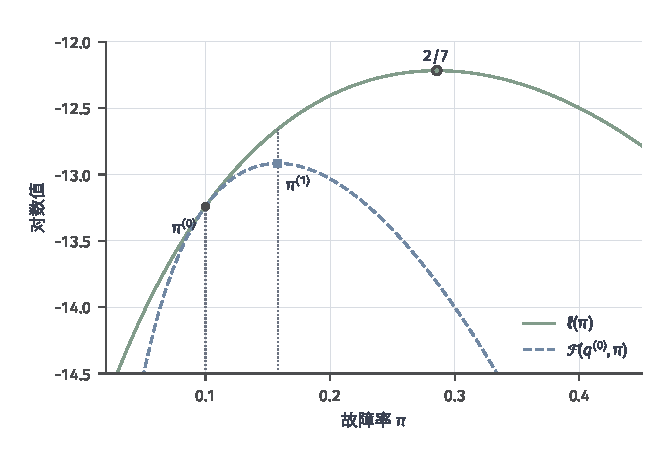
\includegraphics[width=105.412mm]{figures/09-probabilistic-graphical-models/03-learning/matplotlib/pgm-parameter-learning-em-bound/figure.pdf}
  \caption{故障率例子的第一轮EM。实线是观测对数似然，虚线是固定$\pi^{(0)}=0.1$后验所得的下界。两者在旧参数处相等；下界在$\pi^{(1)}\approx0.158044$处最大，而观测似然在$2/7$处最大。图中纵轴为自然对数，曲线可由正文公式直接复算。}
  \label{fig:pgm-parameter-learning-em-bound}
\end{figure}

\begin{figure}[htbp]
  \centering
  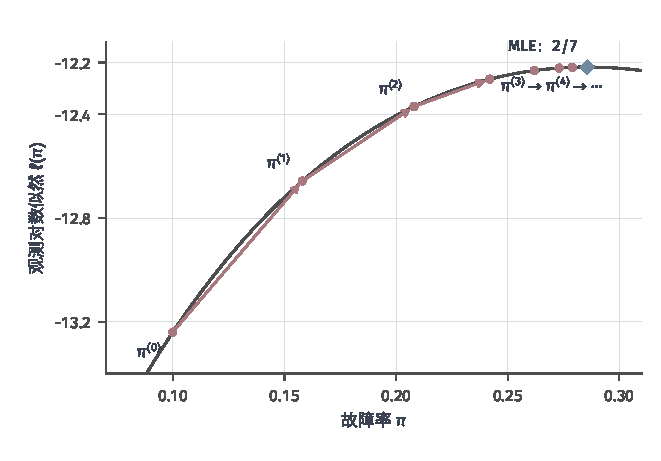
\includegraphics[width=105.412mm]{figures/09-probabilistic-graphical-models/03-learning/matplotlib/pgm-parameter-learning-em-trajectory/figure.pdf}
  \caption{同一标量例子的多轮EM轨迹。红点依次为$\pi^{(0)},\ldots,\pi^{(6)}$，纵坐标均使用观测对数似然而非各轮不同的下界；蓝色菱形是解析MLE $2/7$。该例的轨迹逐轮提高似然并接近解析最优点；一般模型中，单调性定理只保证相邻目标值不下降。}
  \label{fig:pgm-parameter-learning-em-trajectory}
\end{figure}

\subsection{广义EM与近似E步}
\label{sec:pgm-parameter-learning-em-extensions}

定理~\ref{thm:pgm-parameter-learning-em-monotonicity}的M步条件是保持或提高$Q$值。\term{广义EM}（generalized EM, GEM）保留精确E步，只要求M步改进同一个$Q$。例如，对$Q$做带回溯检查的梯度上升，或依次改进几个参数块，只要总更新不降低$Q$，就仍能保证观测似然不下降。步长与参数块更新因此需要检查$Q$的实际变化。

精确EM的E步要求算出真实后验；但在复杂模型里真实后验本身就无法精确求得（这正是第~\ref{chap:pgm-variational}章要处理的推断难题）。既然得不到精确后验，可以退而求其次：只在一个计算得起、又足够灵活的分布族$\mathcal{Q}$里找最接近真实后验的$q$，用它充当E步的结果。如果后验推断本身难以完成，则可以限制$q$属于某个可计算分布族$\mathcal{Q}$。\term{变分EM}（variational EM）在$\mathcal{F}(q,\bm{\theta})$上交替改进近似后验和参数：
\begin{equation}
  \begin{aligned}
    q^{(t+1)}
      &\in\argmax_{q\in\mathcal{Q}}\mathcal{F}(q,\bm{\theta}^{(t)}),\\
    \bm{\theta}^{(t+1)}
      &\in\argmax_{\bm{\theta}\in\Theta}
         \mathcal{F}(q^{(t+1)},\bm{\theta}).
  \end{aligned}
  \label{eq:pgm-parameter-learning-variational-em}
\end{equation}
精确最大化可以放宽为保证同一目标不下降的更新。在固定数据、模型和变分族下，两步都做到这一点，便有
\[
  \mathcal{F}(q^{(t+1)},\bm{\theta}^{(t+1)})
  \geq\mathcal{F}(q^{(t)},\bm{\theta}^{(t)}).
\]
受限后验通常留下非零KL间隙，因此旧点的下界与似然仍可能不同。两步改善给出的是ELBO单调性，观测似然的变化还取决于间隙如何变化\scite{pgm-parameter-learning-neal1998}

更明确地，记$K_t=\sum_j\operatorname{KL}(q_j^{(t)}\,\|\,p_{\bm{\theta}^{(t)}}(\bm{Z}_j\mid\bm{x}_j))$，并简记$\mathcal{F}_t=\mathcal{F}(q^{(t)},\bm{\theta}^{(t)})$，则式~\eqref{eq:pgm-parameter-learning-elbo-identity}给出
\[
  \ell(\bm{\theta}^{(t+1)})-\ell(\bm{\theta}^{(t)})
  =\mathcal{F}_{t+1}-\mathcal{F}_t+K_{t+1}-K_t.
\]
即使第一项非负，后验近似间隙的变化仍可能使总和为负。随机梯度或有噪声的下界估计，还可能连逐步ELBO单调性都不具备。Monte Carlo E步则用有限样本估计$Q$，其更新需控制采样误差，并核查实际改进。

MAP也可以采用EM式更新：E步仍计算给定当前参数的潜变量后验，M步改进$Q(\bm{\theta}\mid\bm{\theta}^{(t)})+\log p(\bm{\theta})$。在对应条件下，单调对象变成$\ell(\bm{\theta})+\log p(\bm{\theta})$，即相差常数的对数后验密度，而非数据似然本身。这个流程输出MAP参数点，完整参数后验的推断将在第~\ref{sec:pgm-parameter-learning-bayesian}节讨论。

\subsection{摊销推断与Wake--Sleep}
\label{sec:pgm-parameter-learning-amortized}

为每条记录、每一轮E步都单独解一个变分优化，在数据量大时代价很高，而且学到的“由观测推断后验”的能力无法在记录之间复用——处理过一万张相似图片后，来了新图片仍要从头优化。摊销推断换个思路：训练一个所有记录共享的映射（识别网络），让它直接吃进观测、吐出近似后验，把逐样本的优化“摊”成一次网络前向计算。变分EM若为每条记录分别保存$q_j$，新记录到来时还要重新求解一个局部优化问题。\term{摊销推断}（amortized inference）改用共享映射$q_{\bm{\phi}}(\bm{z}\mid\bm{x})$，由识别参数$\bm{\phi}$直接把观测映射为近似后验。对固定数据集，可以联合改进
\[
  \mathcal{F}(\bm{\theta},\bm{\phi})
  =\sum_{j=1}^n\mathbb{E}_{q_{\bm{\phi}}(\bm{Z}\mid\bm{x}_j)}
    [\log p_{\bm{\theta}}(\bm{x}_j,\bm{Z})
     -\log q_{\bm{\phi}}(\bm{Z}\mid\bm{x}_j)].
\]
共享映射减少逐样本优化与存储，近似质量可以按三个层次判断。若局部变分族$\mathcal{Q}$不包含真实后验，即使每条记录都求得族内最优$q_j^\star$，仍有由变分族限制带来的近似误差。再用共享映射$q_{\bm{\phi}}(\bm{z}\mid\bm{x})$代替这些逐样本最优解时，所选映射族的最佳结果与各$q_j^\star$之间的目标值差距才是\term{摊销误差}（amortization error），有限网络容量是其来源之一。实际训练若尚未达到该映射族内的最优$\bm{\phi}$，相对于该族最佳映射的剩余差距属于优化误差。具体的梯度估计与重参数化方法见第~\ref{sec:pgm-variational-amortized}节。

\term{Wake--Sleep算法}由Hinton等在1995年为随机Helmholtz机提出。它同时维护自上而下的\term{生成模型}（generative model）$p_{\bm{\theta}}(\bm{x},\bm{z})$与自下而上的\term{识别模型}（recognition model）$q_{\bm{\phi}}(\bm{z}\mid\bm{x})$，但两组参数不在同一个阶段更新。Wake阶段从训练数据取得$\bm{x}$，再由识别模型抽取$\bm{z}$，固定$\bm{\phi}$并更新生成参数$\bm{\theta}$，使这些“数据--解释”对在生成模型下更可能；Sleep阶段固定$\bm{\theta}$，从生成模型自上而下抽取$(\bm{x},\bm{z})$，再更新$\bm{\phi}$，使识别模型能够从生成出的$\bm{x}$恢复对应的$\bm{z}$\scite{pgm-parameter-learning-hinton1995}

这两个方向可以写成不同的总体目标。Wake阶段关于生成参数最大化
\begin{equation}
  J_{\mathrm{wake}}(\bm{\theta};\bm{\phi})
  =\frac{1}{n}\sum_{j=1}^n
    \mathbb{E}_{q_{\bm{\phi}}(\bm{Z}\mid\bm{x}_j)}
      [\log p_{\bm{\theta}}(\bm{x}_j,\bm{Z})],
  \label{eq:pgm-parameter-learning-wake-objective}
\end{equation}
它是固定识别模型后ELBO中依赖$\bm{\theta}$的部分，近似后验的间隙方向为$\operatorname{KL}(q_{\bm{\phi}}(\bm{Z}\mid\bm{x})\,\|\,p_{\bm{\theta}}(\bm{Z}\mid\bm{x}))$。经典算法用$q_{\bm{\phi}}$的样本形成局部随机更新，并不在Wake阶段沿识别参数求这个ELBO的梯度。

Sleep阶段关于识别参数最大化
\begin{equation}
  \begin{aligned}
    J_{\mathrm{sleep}}(\bm{\phi};\bm{\theta})
      &=\mathbb{E}_{p_{\bm{\theta}}(\bm{X},\bm{Z})}
          [\log q_{\bm{\phi}}(\bm{Z}\mid\bm{X})]\\
      &=-\mathbb{E}_{p_{\bm{\theta}}(\bm{X})}
          \operatorname{KL}\bigl(
            p_{\bm{\theta}}(\bm{Z}\mid\bm{X})
            \,\|\,q_{\bm{\phi}}(\bm{Z}\mid\bm{X})\bigr)+C(\bm{\theta}),
  \end{aligned}
  \label{eq:pgm-parameter-learning-sleep-objective}
\end{equation}
其中$C(\bm{\theta})$与$\bm{\phi}$无关。Sleep匹配生成后验到识别分布的KL，方向与Wake的ELBO间隙相反，外层输入又由当前生成模型加权。若生成模型低估真实数据的重要区域，Sleep样本便很少来自这些区域，相应识别映射也缺少训练。

Wake--Sleep的两个阶段因此对应不同目标与输入分布。Wake使用摊销后验更新生成参数，Sleep用生成数据训练识别参数；有限随机更新还包含抽样和求解误差。各阶段的实际目标可以改善，观测数据似然或真实数据ELBO的逐轮变化则需要另行分析，精确EM的单调性证明在这里缺少旧点贴合条件。

\section{观测缺失下的参数学习}
\label{sec:pgm-parameter-learning-incomplete}

除了模型主动引入的潜变量，现实数据还有另一类未观测：某些字段\emph{本应}记录、却因为设备损坏、患者失访、传感器漏报等原因没记下来。这两者都会让对应变量进入“要求和掉的未观测量”，所以边缘化与EM等工具可以复用；但缺失多了一个潜变量没有的问题——\emph{一个值为什么缺失}本身可能携带信息（如病情越重的患者越容易失访），忽略它会导致系统性偏差。观测缺失意味着按设计应记录的数据字段没有全部取得。缺失值与潜变量都形成未观测量，所以第~\ref{sec:pgm-parameter-learning-latent}节的边缘化和近似推断工具可以复用；记录过程若携带缺失值的信息，还要把这一信息纳入模型。本节据此确定如何把缺失字段接入已有推断与学习流程。

\subsection{缺失变量与缺失机制}
\label{sec:pgm-parameter-learning-missingness}

处理缺失数据前，需要先确定一个字段缺失的概率是否取决于它本应取的值。完全随机缺失可以安全忽略；若缺失概率随潜在数值变化，忽略缺失机制会带来偏差。因此要同时建模数据本身和记录状态。以$\bm{Y}$表示本应完整记录的数据向量，$R_i=1$表示$Y_i$已观测，$R_i=0$表示缺失。对一种固定模式$\bm{r}$，把$\bm{y}$拆为$\bm{y}_{\mathrm{obs}}$与$\bm{y}_{\mathrm{mis}}$，拆分位置由$\bm{r}$决定。数据模型为$p_{\bm{\theta}}(\bm{y})$，\term{缺失机制}（missingness mechanism）为$p_{\bm{\psi}}(\bm{r}\mid\bm{y})$，其中$\bm{\psi}$控制记录过程。这一条件分布描述记录概率如何依赖原始值，估计时需要关于采集过程的假设或信息。

可用漏记概率依赖哪些值来判断设备记录机制。设$F,A,S$均已记录，只有$H$可能缺失：独立日志故障对应MCAR，记录概率只依赖已知报警$A$对应MAR；在相同$F,A,S$下，$H$本身仍改变漏报概率时对应MNAR。图~\ref{fig:pgm-parameter-learning-missingness}以这些字段示意机制，具体类别由实际条件依赖决定。

\begin{figure}[htbp]
  \centering
  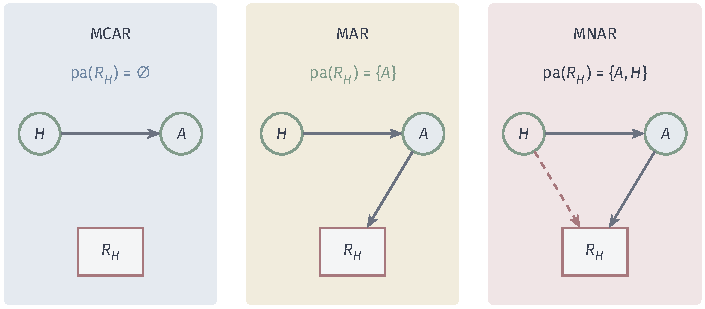
\includegraphics[width=112.000mm]{figures/09-probabilistic-graphical-models/03-learning/tikz/pgm-parameter-learning-missingness/figure.pdf}
  \caption{固定已观测的$F,S$后，温度记录指示量$R_H$的三种示意机制。三栏顶部直接给出$R_H$的父集，底部分别配独立日志故障、报警后安排检查、过热改变漏报概率的日常例子。$A$总是观测，$H$在$R_H=0$时不可见；右图表示给定已观测值后，记录概率仍随$H$变化的MNAR情形；若参数抵消该依赖，类别也随之改变。}
  \label{fig:pgm-parameter-learning-missingness}
\end{figure}

\subsection{可忽略性}
\label{sec:pgm-parameter-learning-ignorability}

MAR条件下，固定实际观测值后，记录概率与待积分的缺失值无关，因而可从积分中提出。对一条记录，观测似然分解为
\begin{equation}
  \begin{aligned}
    L(\bm{\theta},\bm{\psi})
      &=\int p_{\bm{\theta}}(\bm{y})
          p_{\bm{\psi}}(\bm{r}\mid\bm{y})
           \,\mathrm{d}\bm{y}_{\mathrm{mis}}\\
      &=p_{\bm{\psi}}(\bm{r}\mid\bm{y}_{\mathrm{obs}})
        p_{\bm{\theta}}(\bm{y}_{\mathrm{obs}}).
  \end{aligned}
  \label{eq:pgm-parameter-learning-ignorability-factorization}
\end{equation}
参数域可分离为$\Theta\times\Psi$时，关于$\bm\theta$的似然优化可省去机制因子。若还保留参数后验，先验分离$p(\bm\theta,\bm\psi)=p(\bm\theta)p(\bm\psi)$是一组充分条件：机制因子与其先验的积分有限且为正时，积分$\bm\psi$只留下与$\bm\theta$无关的常数。相关先验则可能使该积分仍依赖$\bm\theta$，此时后验需保留它。可忽略性简化的是参数计算，实际缺失字段仍在观测似然中被积分。下一小节据此接入每条记录的可见字段。

\subsection{可忽略缺失下复用未观测变量方法}
\label{sec:pgm-parameter-learning-ignorable-methods}

在可忽略条件下，可以把每条记录实际可见的部分作为$\bm{x}_j=\bm{y}_{j,\mathrm{obs}}$，把缺失部分作为$\bm{z}_j=\bm{y}_{j,\mathrm{mis}}$，直接复用第~\ref{sec:pgm-parameter-learning-latent}节的观测似然、梯度恒等式、精确EM或近似E步。模型若还含主动设置的潜变量$\bm{h}_j$，就把未观测量合并为$\bm{z}_j=(\bm{y}_{j,\mathrm{mis}},\bm{h}_j)$；不同记录可以有不同缺失模式，但每次推断都必须固定该记录实际观测到的分量。

这组记号将两类未观测量接入同一个积分工具，它们在数据获取上的含义仍不同。删除不完整记录会改变拟合所用的记录集合；单次均值或众数填补又省去了条件分布的变动。对离散模型，应计算相关家庭事件的后验期望计数；对高斯模型，还需二阶矩与交叉矩。若采用摊销推断，识别映射还需接收缺失掩码或等价的观测模式信息，以区分真正观测的值和用于输入格式的填充值。

\subsection{不可忽略缺失与可识别性}
\label{sec:pgm-parameter-learning-mnar}

MNAR时，记录过程在给定已观测值后仍依赖缺失值，式~\eqref{eq:pgm-parameter-learning-ignorability-factorization}通常不能分解。此时应为
\[
  p_{\bm{\theta},\bm{\psi}}(\bm{y},\bm{r})
  =p_{\bm{\theta}}(\bm{y})
   p_{\bm{\psi}}(\bm{r}\mid\bm{y})
\]
建立联合模型，把$\bm{R}$作为已观测变量，并对$\bm{Y}_{\mathrm{mis}}$以及原有潜变量共同边缘化。给定这个联合模型后，仍可使用第~\ref{sec:pgm-parameter-learning-latent}节的优化与推断工具；其中的完全数据模型包含采集过程，待估参数也包括$\bm{\psi}$。

联合模型的可识别性仍需检查。不同的数据分布与缺失机制可能诱导同一个$p(\bm{y}_{\mathrm{obs}},\bm{r})$，仅凭现有记录便无法区分它们。对未观测值怎样改变缺失概率的假设，需要由随访数据、外部测量、有效工具变量、受控采集设计或明确的参数约束提供额外信息；缺少这些信息时，可以对未识别的机制假设进行敏感性分析，报告它们对参数和预测的影响。EM负责给定联合模型后的求解，可识别性则由观测信息与模型限制共同决定。

\section{基于分布估计的参数学习}
\label{sec:pgm-parameter-learning-bayesian}

本节通过\term{分布估计}保留参数后验$p(\bm{\theta}\mid\mathcal{D})$，把未知参数本身作为推断变量。它与前面三种数据可见性设定交叉：无未观测变量且满足共轭条件时可能解析更新；含潜变量或缺失值时通常要联合近似参数与未观测变量；得到参数后验后，再通过后验预测把参数不确定性传给新数据。

\subsection{不含未观测变量的共轭后验}
\label{sec:pgm-parameter-learning-conjugacy}

前面的MLE/MAP只用到数据的充分统计量来找一个最优点。贝叶斯方法则要更新参数的整个分布，一个极为方便的情形是共轭：先验和似然属于同一个分布族，相乘后后验仍在该族内，于是学习退化为对少数几个“超参数”做加法更新（先验的虚拟计数 + 数据的真实计数）。不含未观测变量时，局部统计量不仅能用来找最优点，也能更新参数分布。\term{共轭先验}（conjugate prior）是与似然相乘后仍留在同一分布族中的先验，因此可通过更新有限组超参数表示整个后验。

对一个独立参数块$\bm{\eta}$，假设其似然中与参数有关的部分具有形式
\[
  p(\mathcal{D}_b\mid\bm{\eta})
  \propto\exp\{\bm{\eta}^\top\bm{S}_b-n_ba(\bm{\eta})\},
\]
其中$\bm{S}_b$是聚合充分统计量，$n_b$是该块的观测次数，$a$是对应对数归一化函数。若采用相对于指定参数测度、可归一化的先验$p(\bm{\eta}\mid\bm{\chi},\nu)\propto\exp\{\bm{\eta}^\top\bm{\chi}-\nu a(\bm{\eta})\}$，则
\begin{equation}
  p(\bm{\eta}\mid\mathcal{D}_b)
  \propto
  \exp\{\bm{\eta}^\top(\bm{\chi}+\bm{S}_b)
                 -(\nu+n_b)a(\bm{\eta})\}.
  \label{eq:pgm-parameter-learning-conjugate-update}
\end{equation}
指数相加给出$\bm{\chi}\leftarrow\bm{\chi}+\bm{S}_b$与$\nu\leftarrow\nu+n_b$。这一写法适用于拥有共同归一化函数的参数块，例如离散CPT的一行；一般条件指数族的归一化函数还依赖父节点值，需要按实际设计逐记录保留这些项。

在所有节点均已观测、没有参数共享且先验也按节点和CPT行独立分解时，似然的分解使后验同样局部分解：
\begin{equation}
  p(\bm{\theta}\mid\mathcal{D})
   =\prod_{i,a}
     \operatorname{Dirichlet}
       (\bm{\theta}_{i,a};
        \bm{\alpha}_{i,a}+\bm{N}_{i,a}).
  \label{eq:pgm-parameter-learning-local-posterior}
\end{equation}
数据沿图结构的作用在这里很具体：每条记录只给各节点家庭的相应单元格增加计数。父配置从未出现时，该行后验保持先验，反映这一局部条件尚未得到数据更新。对完整的线性高斯局部回归，适当的正态与逆Gamma联合先验也可以利用设计矩阵的交叉乘积解析更新，原理同样是聚合局部充分统计量\scite{pgm-murphy2012}

Dirichlet后验保留了整行概率的不确定性，而不只给出式~\eqref{eq:pgm-parameter-learning-cpt-map}的众数。记$\alpha_{i,a,0}=\sum_k\alpha_{i,a,k}$，则
\begin{equation}
  \mathbb{E}[\theta_{i,a,k}\mid\mathcal{D}]
    =\frac{N_{i,a,k}+\alpha_{i,a,k}}
            {N_{i,a}+\alpha_{i,a,0}}.
  \label{eq:pgm-parameter-learning-dirichlet-estimates}
\end{equation}
这个后验均值只需正超参数便定义良好，它将整个参数后验压缩成一个点，分布的宽度仍需其他摘要或完整后验来表达。均匀Dirichlet先验下，式~\eqref{eq:pgm-parameter-learning-cpt-map}的内部MAP与MLE相同，常见的加一平滑则来自本式的后验均值。

后验是否局部分解取决于似然和先验共同的结构。共享超参数会将原来独立的块联系起来，缺失数据的求和也通常打破式~\eqref{eq:pgm-parameter-learning-local-posterior}。EM的一轮期望计数依赖当前参数点，用于更新下一参数点。要保留参数不确定性，则需联合推断$p(\bm{\theta},\bm{z}_{1:n}\mid\mathcal{D})$；仅将该期望计数代入Dirichlet更新会得到一种额外近似。

设备例子也能展示后验保留了多少信息。表~\ref{tab:pgm-parameter-learning-device-counts}给出$5$次故障和$15$次正常，结合$\operatorname{Beta}(2,2)$先验得到$\pi\mid\mathcal{D}\sim\operatorname{Beta}(7,17)$。同一份数据的MLE、MAP与后验均值分别为$1/4$、$3/11$和$7/24$；前两者是不同目标的最优点，第三个数只是后验的一项摘要。该后验的方差为
\[
  \operatorname{Var}(\pi\mid\mathcal{D})
   =\frac{7\times17}{24^2\times25}
   =\frac{119}{14400}\approx0.008264.
\]
后验方差保留了故障率的剩余不确定性，$7/24$只概括其中心。新增完整记录时继续累加成功、失败计数即可，先验超参数则记录建模选择。

\subsection{含未观测变量的近似后验}
\label{sec:pgm-parameter-learning-approximate-posterior}

9.5.1的共轭更新之所以能解析完成，依赖“所有变量都观测、各参数块独立”这两个条件。一旦有潜变量或缺失值，参数后验就不再能与未观测量分开：看到数据后，“参数是多少”和“潜变量取什么”相互影响，必须联合推断，干净的计数加超参更新也随之失效。一旦含有潜变量或缺失值，参数后验通常要与未观测变量联合推断；非共轭局部模型和复杂参数共享还会进一步破坏解析形式。此时可以沿用第~\ref{chap:pgm-variational}章和第~\ref{chap:pgm-sampling}章的方法，其推断对象扩展为参数与状态的联合分布。以下用$\bm{z}_{1:n}$统称各条记录中的潜变量和实际缺失字段。对MNAR，$\mathcal{D}$还包含已观测的缺失指示，缺失机制参数$\bm{\psi}$也属于联合后验；为显式保留这一情形，下面的公式写出$\bm{\psi}$，不含缺失机制或机制可忽略时则删去所有$\bm{\psi}$项。

变分方法选取$q_{\bm{\phi}}(\bm{\theta},\bm{\psi},\bm{z}_{1:n})$，优化
\begin{equation}
  \begin{aligned}
    \mathcal{L}(\bm{\phi})
      &=\mathbb{E}_{q_{\bm{\phi}}}
       [\log p(\mathcal{D},\bm{z}_{1:n},\bm{\theta},\bm{\psi})
        -\log q_{\bm{\phi}}
          (\bm{\theta},\bm{\psi},\bm{z}_{1:n})],\\
    \log p(\mathcal{D})
      &=\mathcal{L}(\bm{\phi})
        +\operatorname{KL}\bigl(
          q_{\bm{\phi}}\,\|\,
          p(\bm{\theta},\bm{\psi},\bm{z}_{1:n}\mid\mathcal{D})
        \bigr).
  \end{aligned}
  \label{eq:pgm-parameter-learning-bayesian-elbo}
\end{equation}
这里数据参数$\bm{\theta}$与机制参数$\bm{\psi}$的先验都已进入联合分布，两者也都在证据中被积分；$\log p(\mathcal{D})$在模型和超参数固定时是常数。不含$\bm{\psi}$时，公式退化为只对数据参数与状态推断。此处优化近似分布参数$\bm{\phi}$，证据固定；变分EM则优化模型参数$\bm{\theta}$及状态近似，观测似然随$\bm{\theta}$变化。常用因子化假设可以降低计算量，却可能遗漏参数间相关性或后验的多个峰；下界求解的误差与分布族的表达误差需分别检查。

在共轭的变分更新中，期望计数确实可能作为超参数出现，但那属于特定变分族下的坐标更新。相应局部状态更新通常使用$\exp\{\mathbb{E}[\log\theta_{i,a,k}]\}$，而不是把后验均值代入$\theta$；一般有$\mathbb{E}[\log\theta]\ne\log\mathbb{E}[\theta]$。这些局部更新由各自目标导出，EM的点参数、贝叶斯变分的期望对数以及平滑计数对应不同计算。

MCMC则构造以参数后验或参数与潜变量联合后验为平稳分布的链，用其样本近似积分。若只关心普通可计算似然，后验中与参数无关的证据常数会在Metropolis--Hastings比率中约掉；无向模型的$Z(\bm{\theta})$却依赖候选参数，通常不会消失。这类模型可能仍需额外的内层推断或专门的采样构造。有限运行的积分精度还取决于混合、多峰之间的移动和查询相关的有效样本量，应结合相应诊断报告。

若后验在一个内部峰附近集中，还可以用\term{拉普拉斯近似}（Laplace approximation），即用峰值附近的二次曲率构造高斯分布。记$g(\bm{\theta})=\log p(\bm{\theta}\mid\mathcal{D})$，在局部MAP点$\widehat{\bm{\theta}}$作二阶展开；若$\bm{H}=-\nabla^2g(\widehat{\bm{\theta}})$正定，则
\[
  p(\bm{\theta}\mid\mathcal{D})
    \approx\mathcal{N}(\bm{\theta};
          \widehat{\bm{\theta}},\bm{H}^{-1}).
\]
边界峰、明显偏斜、多峰或不可识别方向会破坏这一局部高斯描述。对有约束的参数，宜先选择适当坐标，并将密度变换的Jacobian纳入目标，使曲率与MAP对应所用坐标的密度。比较这三类方法时，可以报告具体后验量或预测量的误差，以及相应计算预算。

\subsection{后验预测}
\label{sec:pgm-parameter-learning-posterior-predictive}

学出参数分布后做预测，要同时考虑两层不确定性：即使参数已知，新设备是否故障仍是随机的；而参数本身我们也不完全确定。后验预测把这两层一起积分掉，因此通常比直接代入单个参数估计的插件预测更保守、更能反映有限数据下的不确定性。得到参数后验后，新设备的状态仍具有随机性，而故障率本身也不完全确定。\term{后验预测}（posterior predictive）将这两种不确定性合并：在每个可能参数下计算新观测的分布，再按参数后验加权，
\begin{equation}
  p(\bm{x}_*\mid\mathcal{D})
   =\int p_{\bm{\theta}}(\bm{x}_*)
            p(\bm{\theta}\mid\mathcal{D})\,\mathrm{d}\bm{\theta}.
  \label{eq:pgm-parameter-learning-posterior-predictive}
\end{equation}
若预测还涉及新潜变量，应在内层同时消去它们。\term{插件预测}（plug-in prediction）则把某个点估计$\widehat{\bm{\theta}}$代入$p_{\bm{\theta}}(\bm{x}_*)$，计算较简单，但忽略了参数分布的宽度。

对单台设备的Bernoulli故障变量，后验预测恰好等于代入后验均值的结果：$p(F_*=1\mid\mathcal{D})=\mathbb{E}[\pi\mid\mathcal{D}]=7/24$。单设备故障概率对$\pi$线性，因此该查询仅需要一阶矩。其他查询还可能涉及更高阶矩。考虑两台在给定$\pi$后独立的新设备，则
\[
  \begin{aligned}
    p(F_{*,1}=1,F_{*,2}=1\mid\mathcal{D})
      &=\mathbb{E}[\pi^2\mid\mathcal{D}]
        =\frac{7\times8}{24\times25}
        =\frac{7}{75},\\
    p_{\mathrm{plug}}(F_{*,1}=1,F_{*,2}=1)
      &=(7/24)^2=\frac{49}{576}.
  \end{aligned}
\]
两者约为$0.09333$和$0.08507$，相差$\operatorname{Var}(\pi\mid\mathcal{D})$。积分共同参数后，两台设备不再后验预测独立：它们都受到同一故障率未知性的影响。对未来$m$台设备的故障数，完整预测服从Beta--二项分布，参数混合使其与固定平均故障率的二项分布不同。

条件预测还要说明新输入怎样被处理。纯条件模型把$\bm{x}_*$视为给定设计，使用$\int p_{\bm{\theta}}(\bm{y}_*\mid\bm{x}_*)p(\bm{\theta}\mid\mathcal{D})\,\mathrm{d}\bm{\theta}$。若训练的是联合生成模型，新输入本身也能提供参数信息，则严格的条件后验预测为
\[
  p(\bm{y}_*\mid\bm{x}_*,\mathcal{D})
  =\frac{\int p_{\bm{\theta}}(\bm{x}_*,\bm{y}_*)
                      p(\bm{\theta}\mid\mathcal{D})\,\mathrm{d}\bm{\theta}}
         {\int p_{\bm{\theta}}(\bm{x}_*)
                      p(\bm{\theta}\mid\mathcal{D})\,\mathrm{d}\bm{\theta}}.
\]
等价地，它用$p(\bm{\theta}\mid\mathcal{D},\bm{x}_*)$加权条件分布。只有在输入不更新相关参数等条件下，才能直接改用训练后的参数后验作权重。预测对象不同，所需的积分顺序与权重也可能不同。

\section{学习算法分析}
\label{sec:pgm-parameter-learning-analysis}

学出一组参数并不等于得到一个可靠模型：算法可能没把目标优化到位，模型族本身可能表达不了真实分布，即便两者都好，有限数据上学到的也未必适用于新记录。因此评价学习结果要分三个层次，它们对应三类不同来源、不能互相弥补的差距。学习结果可以从三个层次分析。表达能力考察固定图与局部分布族能否表示所需的观测分布，参数共享、潜变量和可识别性决定哪些差异可由模型表达并由数据区分。收敛性考察实际更新是否接近所选目标的最优候选、达到何种驻点，以及推断误差和计算规模如何影响求解速度。泛化性则考察从有限训练记录选择的候选能否预测新记录，重点是独立测试分布、参数不确定性和模型失配。以下在学习所需统计量、优化过程及结果评价中分别落实这三个问题。

\subsection{学习与推断的耦合}
\label{sec:pgm-parameter-learning-inference-coupling}

先从模型表达与学习所需的信息看各节的差异。固定图及局部分布族限定了候选分布：缺少必要的相互作用或使用不合适的局部族时，即使求解充分，也可能无法拟合目标观测分布。在这一族内，各种数据设定又提供不同统计量。观测完整且不含潜变量的有向图已经给出局部事件，独立参数块只需聚合计数或回归矩；联合无向图虽然观测完整，仍需计算全局归一化带来的模型期望；条件无向图需要对每个输入计算输出条件分布的期望；含潜变量或缺失值时，还要计算每条记录条件下的后验期望。若联合无向图同时含有潜变量，两类推断任务会同时存在。

例如，对充分统计量为$\bm{T}(\bm{x},\bm{z})$的无向指数族潜变量模型，平均观测似然梯度为
\begin{equation}
  \begin{aligned}
    \frac{1}{n}\nabla_{\bm{\theta}}\ell
      &=\frac{1}{n}\sum_{j=1}^n
        \mathbb{E}_{p_{\bm{\theta}}(\bm{Z}\mid\bm{x}_j)}
          [\bm{T}(\bm{x}_j,\bm{Z})]\\
      &\quad-\mathbb{E}_{p_{\bm{\theta}}(\bm{X},\bm{Z})}
          [\bm{T}(\bm{X},\bm{Z})].
  \end{aligned}
  \label{eq:pgm-parameter-learning-two-expectations}
\end{equation}
第一项问的是“这条观测记录可能来自哪些状态”，第二项问的是“模型不附加证据时会产生哪些状态”。第一项需要附加该记录证据的样本，第二项需要模型无证据的样本。两种期望共同进入参数梯度，因此后验易算的E步仍可能伴随配分函数难算的M步。

学习的内层推断成本随图结构变化。离散完整有向图可以一次扫描累加家庭计数，但表格存储量约为$\sum_i r_i\prod_{v\in\operatorname{pa}(i)}r_v$，高入度节点仍可能很贵。对最大状态数为$r$、诱导宽度为$w$的离散精确消元，主要因子运算规模通常含$r^{w+1}$；潜变量学习还要针对不同证据重复或批量复用这些运算。图固定时可以复用消元结构与消息调度，但参数更新后消息数值一般需要重算。相关算法见第~\ref{chap:pgm-elimination}章和第~\ref{chap:pgm-junction-tree}章。

\subsection{优化与可扩展性}
\label{sec:pgm-parameter-learning-scalability}

收敛速度的判断需要同时计算每轮成本与达到所需目标差距的轮数。样本数很大时，遍历全部记录可能成为每轮的主要成本。\term{随机梯度}（stochastic gradient）从小批量记录估计全数据梯度。若优化平均对数似然，大小为$b$的均匀小批量$\mathcal{B}$给出$b^{-1}\sum_{j\in\mathcal{B}}\nabla\log p_{\bm{\theta}}(\bm{x}_j)$；若优化总和目标，则相应乘以$n$。先验在总和目标中只出现一次；把整个目标除以$n$改成均值时，正则项也应同步除以$n$，以保持原有先验与数据的相对权重。

小批量降低经验项的每轮成本，内层推断仍决定更新的准确性。可把实际更新使用的梯度写成
\[
  \widehat{\bm{g}}^{(t)}
   =\nabla J(\bm{\theta}^{(t)})
      +\bm{b}_{\mathrm{inf}}^{(t)}
      +\bm{\xi}^{(t)},
\]
其中$\bm{b}_{\mathrm{inf}}^{(t)}$表示近似推断带来的系统偏差，$\bm{\xi}^{(t)}$表示中心化后的抽样波动。增加批量主要降低波动，固定步数链或受限变分族的系统偏差则需要改变内层求解来控制。偏差随参数变化时，更新可接近一个偏移后的平衡点，平滑训练曲线本身不足以识别原似然驻点。

参数共享减少自由度，同时限制候选分布；它也能汇集多个位置的数据以估计罕见配置。共享后，式~\eqref{eq:pgm-parameter-learning-dag-likelihood}虽仍是局部项之和，同一参数的梯度要从所有出现位置累加。同一大图上的模板实例通常相关，聚合它们时仍需保留模型内部依赖；独立设备或独立序列才提供相应的跨记录独立性。

\term{自动微分}（automatic differentiation）沿计算图应用链式法则，可同时处理共享参数与复杂局部网络；所得导数对应所写的计算目标。若反向传播穿过固定次数的消息更新，所得导数针对这个有限计算过程，与精确似然导数的差距需由推断近似分析。EM的M步则应固定E步分布，对$Q$中的新参数求导；梯度穿过旧后验构造时会多出另一组依赖项，形成不同更新。归一化项与后验期望的计算精度，仍决定上述导数与统计目标梯度的差距。

非凸点估计还依赖初始化。不同初值可能把EM、变分学习或一般梯度法送入不同的吸引区域，多次初始化可以比较这些区域内的目标值和预测表现，所得最好结果仍只在已探索区域内成立。潜变量未观测所留下的信息不足，还可能使参数与期望统计量调整缓慢，应结合目标变化与求解条件判断停止，而非仅看参数位移。

优化目标本身也可能没有有限最大值。高斯混合模型中，若一个$m$维分量保持固定正权重，把均值移到某个样本$\bm{x}_j$上，并令协方差为$\varepsilon^2\bm{I}$，该点密度正比于$\varepsilon^{-m}$。只要其他分量仍给其余样本正密度，令$\varepsilon\to0$就可使总似然无界。这种\term{退化解}（degenerate solution）来自目标的无界边界路径，沿该路径继续提高似然会缩小协方差，而无法到达有限参数最优点。对协方差加下界或采用适当先验可以排除相应路径，但这会改变原来的无约束MLE问题。

当训练集上的表现不理想时，盲目“再多迭代一会儿”未必有用，因为差距可能根本不来自优化没收敛。把误差按来源拆开，才能对症下药：数据不够、推断不准、优化不足需要完全不同的补救。收敛诊断还需区分目标误差来自何处。\term{统计误差}（statistical error）来自有限数据，即使精确求出样本目标的最优解，也未必接近总体最优参数；\term{推断误差}（inference error）来自近似边缘、期望或积分；\term{优化误差}（optimization error）则是相对于所选目标尚未充分求解的差距。模型族与真实分布的差异另产生表达或设定偏差。它们通常不在参数空间简单相加，但针对的计算不同：更多独立数据减少统计不确定性，改进内层推断控制近似偏差，继续优化减少当前目标的求解差距。

\subsection{学习结果的评价}
\label{sec:pgm-parameter-learning-evaluation}

预测新记录时，训练样本的数量与局部配置覆盖决定可用于估计的信息，图结构、参数共享和正则化则限制所选候选的自由度。罕见父配置可能只有少量记录，因而其参数仍有较大不确定性；共享或先验可借助其他信息，却也引入相应限制。训练和测试来自不同设备群体或采集机制时，还需检查这些限制及概率关系是否适用于新记录。以下评价分别检验参数解释、独立预测和模型失配。

解释参数时，先区分候选分布与其参数表示。若不同参数产生相同观测分布，就存在\term{不可识别性}（non-identifiability）；增加观测数量也只能确定该等价类。交换混合分量的编号并同时交换其权重与局部参数，观测分布不变，这称为\term{标签交换}（label switching）；因子模型的某些旋转、无向势函数的常数重分配以及MNAR模型中数据分布与缺失机制的抵消也会产生不唯一性。约束可以选定一个代表，外部信息可能恢复识别，这些选择的作用取决于所加信息。预测评价可优先报告可识别的量或重标记不变的结构，任意参数代表的机制解释则需要额外识别条件。

泛化性关注新记录，而训练似然描述整批训练数据的概率或密度。条件模型对应给定输入后的训练标签概率。MAP、ELBO或替代准则的改善具有各自目标含义，评价新记录时应另外计算所需的预测分数。要判断概率模型能否预测新记录，应使用未参与训练和调参的独立测试集；记录具有分组或时间依赖时，划分也应避免同一设备或未来信息泄漏到训练侧。测试平均预测对数似然可以写为
\[
  \frac{1}{n_{\mathrm{test}}}
  \sum_{j=1}^{n_{\mathrm{test}}}
    \log p_{\mathrm{pred}}(\bm{x}^{\mathrm{test}}_j).
\]
条件模型应改用对应的条件预测概率，缺失数据应使用实际观测部分的概率及所声明的缺失机制。比较分数时，应固定联合或条件查询以及连续变量的坐标和单位，使数值对应同一预测任务。

用ELBO评估时，所报告的量是预测对数似然的下界。不同模型或不同近似族的下界间隙可能不同，排名也可能受到影响。无向模型还需估计$Z$才能将能量转成概率；伪似然和CD指标也分别衡量其局部准则或有限步更新，归一化测试似然需要另行计算。报告应说明归一化、积分或采样近似所用的方法与误差来源。

对数似然衡量整份概率分配，还可以单独检查概率是否与实际频率吻合。\term{概率校准}（probability calibration）要求预测某事件概率约为$u$的记录中，该事件发生比例也约为$u$。对故障预测，可在独立记录上按预测概率分箱，比较每箱平均概率与故障频率，并同时报告箱内样本量或不确定性。箱内记录很少时，频率偏差可能来自抽样波动。恒定预测总体故障率也可校准，但缺少区分高风险与低风险的能力，因此还需结合区分能力和预测对数似然评价。

参数后验还支持更有针对性的模型检查。\term{后验预测检查}（posterior predictive check）从后验预测中生成与原数据设计相同的重复数据，再比较具有实际意义的统计量。例如，设备模型可以比较总报警率、各故障组的过热率，以及给定$H,S$后报警与故障之间是否仍有模型没有解释的关联。若研究对象包含缺失过程，复制数据时也应模拟相应记录机制，或明确固定了什么观测设计。观测统计量偏离后验预测的主要概率区域时，提示模型结构、局部分布或先验可能不适合当前数据。

后验预测检查定位已观察数据与模型的哪些统计特征不相容。它复用了拟合数据，所提供的是模型诊断；新数据上的泛化证据仍来自适当独立的预测评价。检查范围也取决于所选统计量，未被检查的结构可能仍有失配。积分参数得到的模型证据、比较两个证据之比的Bayes因子，以及BIC，主要服务于模型或结构比较，且需要考虑先验与正则条件。第~\ref{sec:pgm-structure-learning-scores}节将给出它们的定义，并说明这种比较与参数拟合、预测评价的区别。

\section{本章小结}
\label{sec:pgm-parameter-learning-summary}

本章从“模型给定”走向“从数据确定模型”，在图结构固定的前提下学习局部概率参数。贯穿全章的是开篇提出的两条正交主线。第一条是数据可见性：完整可见的有向模型可直接聚合计数或回归矩，是最容易的情形；无向模型因全局归一化，即使数据完整也要在学习内层反复计算模型期望；潜变量和缺失字段则进一步要求用后验期望（软计数）代替真实计数，使学习与推断深度耦合，而缺失字段还要额外考察记录机制是否携带信息。第二条是估计方式：MLE与MAP输出一个参数点，分布估计则保留整个参数后验，并通过后验预测把参数不确定性传入对新记录的预测。两条轴相互正交、可以组合。

算法结论应对应实际目标。精确EM用贴合下界推出观测似然不下降，GEM允许M步只改进同一$Q$；变分EM的两步改进对应ELBO，Monte Carlo E步还需控制抽样误差。Wake与Sleep分别更新不同分布下的目标，其变化需要按阶段解释。

表达能力由固定图、局部分布和参数约束限定；收敛性受目标形状、初始化、内层推断和计算规模影响；泛化性则需用新记录上的预测分数、校准及参数不确定性检验。模型诊断、求解诊断和独立预测评价提供不同证据，可识别性与退化边界决定这些结果能够如何解释。

\paragraph{扩展阅读}
Bishop的PRML第9章将完整数据估计、潜变量与EM联系起来；Koller与Friedman的教材补充图模型中的充分统计量和缺失机制。阅读时可将每种方法的观测似然、辅助目标及可识别条件逐项对应，理解目标改善如何转化为学习结论\scite{bishop2006,pgm-koller2009}

\chapter{结构学习}
\label{chap:pgm-structure-learning}

前一章把图的结构（哪些变量相连、边朝哪个方向）视为专家或设计给定的前提，只从数据估计局部条件分布的参数。实际数据往往没有提供可靠结构：只有设备运行记录时，故障、过热、报警和传感器之间的直接关系仍待确定。\emph{结构学习}研究如何根据数据和领域知识选择或评价这些连接。

结构学习比参数学习多了两类困难。第一，选择空间巨大且离散：参数学习在连续参数空间中优化，结构则要在$2^{\binom d2}$种边集中挑选，节点数稍多就不能逐一尝试。第二，观测数据通常只能把结构确定到一个等价类：若干箭头方向不同的图可以产生相同的观测分布，仅凭观测数据无法取舍。还要区分两个层次：连出一张能拟合数据、表示变量依赖的图，与把箭头解释成故障传播那样的因果方向并不相同；后者需要额外的机制假设或实验信息。

本章沿三类工具展开。\emph{条件独立检验}判断给定其他变量后两个变量是否仍相关，提供关于边是否存在的局部证据；\emph{评分}把整张图作为候选，用拟合程度与结构复杂度的平衡给出可比较的分数；\emph{搜索}根据这些证据在合法图空间中寻找高分候选。缺失观测和潜变量会改变可用证据。本章最后说明，仅有观测分布通常不足以把箭头解释为因果作用，还需要干预数据或额外的函数与噪声假设。

\section{结构学习的定义}
\label{sec:pgm-structure-learning-definition}

本节固定结构学习的对象、可能的输出形式和观测等价这一根本限制。记节点集合为$V=\{1,\ldots,d\}$，随机向量为$\bm{X}=(X_1,\ldots,X_d)^{\top}$，数据为$\mathcal{D}=\{\bm{x}_r:r=1,\ldots,n\}$，暂取样本独立同分布。给定候选图族$\mathfrak{G}$及各图对应的分布族$\mathcal{M}(\mathcal{G})$，\term{结构学习}（structure learning）利用数据和领域知识选择或评价依赖关系的图表示。候选范围可以规定边的类型，也可以限制父集大小、禁止特定边或仅允许树；缺失数据及多干预环境随后另行处理。

学习结果应表示数据能够确定的信息。用于预测时，可以选择拟合与复杂度折中的图；保留不确定性时，可以给出结构后验；高斯条件依赖可以用稀疏精度矩阵表示。若多张图在可用信息下无法区分，结果就应保留它们的共同关系。这些输出对应不同统计目标，并非把同一个确定结果换一种画法。

结构学习通常不能从纯观测数据中唯一恢复一张带确定箭头的图。有向图通过d-分离编码独立性；d-分离关系完全相同的不同有向无环图，即使箭头方向不同，也能表示同一批条件独立关系并拟合同一族分布，因此在观测数据下无法区分。具有相同d-分离关系的有向无环图组成\term{Markov等价类}（Markov equivalence class, MEC），“等价”指它们在纯观测数据下不可区分。两图等价要求两件事：一是忽略方向后相邻关系完全相同，即\term{骨架}（skeleton）相同；二是$i\to k\leftarrow j$且$i,j$本身不相邻的\term{无屏蔽碰撞结构}（unshielded collider，又称v-structure）也相同。碰撞结构是唯一能仅凭独立性模式判断方向的局部结构，对撞点处的条件化会打开路径。这里比较图所蕴含的全部独立关系，区别于特定参数取特殊值时靠数值抵消偶然产生的额外独立性；完整刻画见图模型教材\scite{pgm-koller2009}

局部条件分布没有额外函数形式限制时，等价图表示相同的分布族。例如$X_1\to X_2\to X_3$、$X_1\leftarrow X_2\leftarrow X_3$和$X_1\leftarrow X_2\to X_3$都只要求$X_1\perp X_3\mid X_2$。将两条边同时指向$X_2$则得到碰撞图，它要求两端边缘独立，属于另一个等价类。图~\ref{fig:pgm-structure-learning-equivalence}对照这些方向，展示三种表示共同确定的关系。

等价类包含多张图，逐一列出会造成冗余，也可能使某个代表图的方向被误认为由数据唯一确定。部分有向图只画出类内一致认同的方向：方向在类内可以翻转的边保留为无向边。\term{完成的部分有向无环图}（completed partially directed acyclic graph, CPDAG）把等价类共同确定的方向画成箭头、其余边画成无向边，也称观测本质图。未定向边的合法选择相互约束：补全必须保持无环且不增加无屏蔽碰撞。因此，“恢复CPDAG”表示恢复类内不变的关系；任取代表图所增加的方向仍属选择，而非新增数据证据。

\begin{figure}[!t]
  \centering
  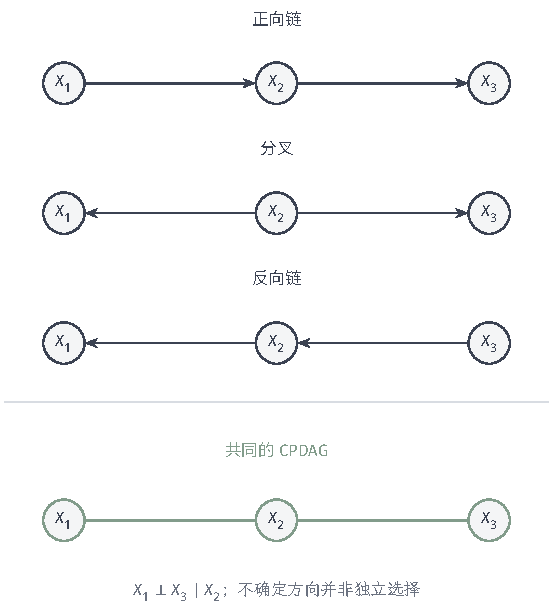
\includegraphics[width=93.652mm]{figures/09-probabilistic-graphical-models/03-learning/tikz/pgm-structure-learning-equivalence/figure.pdf}
  \caption{三种无碰撞有向图的等价表示。它们的骨架及条件独立关系相同，底部CPDAG保留这些共同信息；无向边表示类内方向可变。定向时两边须共同考虑：若都指向$X_2$，就会引入新碰撞，离开原等价类。}
  \label{fig:pgm-structure-learning-equivalence}
\end{figure}


候选空间决定结构搜索的计算规模。$d$个节点共有$2^{\binom d2}$种简单无向图；有向无环图即使固定一个拓扑序，也有这么多种边集可选，而拓扑序本身还有$d!$种排列。十几个节点时，候选图数量已经排除了暴力枚举，后续搜索算法需要在巨大空间中依据检验证据或评分作取舍。潜变量边缘化后的混合图允许不同端点标记，还受到整体合法性约束。扩大图族会增加可表示的分布，也增加参数、样本和搜索需求。频繁推断时，可把树宽等计算性质列为候选限制，并说明它们来自计算预算。

\section{有向图结构学习}
\label{sec:pgm-structure-learning-directed}

有向图结构学习使用两类性质不同的证据，再由搜索步骤组织比较。条件独立检验考察局部联系，似然及复杂度评分为整张图打分。搜索算法根据一种或两类证据寻找候选。检验和评分规定怎样比较结构，搜索规定怎样执行比较。检验是局部的：它一次只回答一对变量在给定某集合后是否独立；评分是整体的：它给每张候选图一个综合分数，同时考虑拟合与复杂度。

\subsection{条件独立约束}
\label{sec:pgm-structure-learning-constraints}

由条件独立检验删边依赖忠实性假设：数据中观察到的独立性应与图上的d-分离对应。即使两个变量在图上有边，具体条件概率参数也可能取特殊数值，使相关在数值上抵消而产生额外独立；这种独立来自参数巧合，不反映结构性质。\term{忠实性}（faithfulness）假设要求分布的条件独立与图上的d-分离一致，即独立只能来自图结构、不能来自参数抵消。若集合$S\subseteq V\setminus\{i,j\}$使$X_i$与$X_j$条件独立，在该假设下可删去$i,j$之间的边。总体分布未知时，算法实际检验的是
\[
  H_0:X_i\perp X_j\mid\bm{X}_S,
\]
并在未拒绝$H_0$时暂时删边。有限样本的检验功效会限制这一步：真实依赖过弱时也可能未被检出，因此未拒绝只是当前证据，尚未证明独立。

那么对离散数据，具体怎样检验“给定$\bm X_S$后$X_i$与$X_j$是否独立”？思路是比较两张计数表：一张是数据里实际观察到的$(X_i,X_j)$在各层$S$下的联合频率，另一张是假设两者独立时理应出现的频率（边缘频率相乘）。两者吻合则独立成立，差异越大越说明有直接依赖。离散记录可以按条件配置分层计数。令$N_{a,b,s}$统计$(X_i,X_j,\bm{X}_S)=(a,b,s)$的次数，点号表示对相应指标求和。比较联合频率与独立假设下的频率，得到似然比统计量
\begin{equation}
  G^2=2\sum_{a,b,s:N_{a,b,s}>0}
  N_{a,b,s}\log
  \frac{N_{a,b,s}N_{\cdot,\cdot,s}}
       {N_{a,\cdot,s}N_{\cdot,b,s}}.
  \label{eq:pgm-structure-learning-g-test}
\end{equation}
各单元概率为正、状态数固定且样本足够时，原假设下的统计量渐近服从卡方分布。若条件变量有$q_S$种配置，自由度为$q_S(r_i-1)(r_j-1)$，$r_i,r_j$是两端状态数。结构性零单元、稀有配置及小样本都可能破坏近似，检验校准需与这些条件一起检查。

上面的似然比检验还可以换一个更直观的信息论量来表达：它衡量“知道$X_j$以后，对$X_i$的不确定性平均能减少多少”。\term{条件互信息}（conditional mutual information）就是这个量，它比较条件联合分布与条件边缘乘积之间的差距；有限离散情形为
\[
  I(X_i;X_j\mid\bm{X}_S)
  =\sum_{a,b,s}p(a,b,s)
       \log\frac{p(a,b\mid s)}{p(a\mid s)p(b\mid s)}.
\]
正概率项构成各条件配置下KL散度的加权平均，故此量非负，且为零恰好表示条件独立。代入经验频率可得$\widehat I=G^2/(2n)$。$S$为空时，它成为\term{互信息}（mutual information），衡量边缘依赖；这种依赖可能通过其他变量传递，未必对应直接边。

联合高斯分布提供了另一个计算入口。分别将两端对$\bm{X}_S$作线性回归，残差的相关系数就是偏相关$\rho_{i,j\mid S}$；在非退化高斯设定中，它为零等价于条件独立。对样本偏相关$\widehat\rho$作Fisher变换，得到
\[
  Z=\frac{\sqrt{n-|S|-3}}{2}
    \log\frac{1+\widehat\rho_{i,j\mid S}}
                  {1-\widehat\rho_{i,j\mid S}},
\]
在原假设$\rho_{i,j\mid S}=0$下，取$n>|S|+3$且相应渐近近似适用时，$Z$近似服从标准正态分布。非高斯数据中的零偏相关只排除某类线性关系，需要更丰富的统计信息才能检验条件独立。核检验可用于非线性关系，其结论仍依赖核、正则化及零分布校准；一般回归残差不相关也不足以替代原变量条件独立。

下面用同一张计数表比较检验、评分和搜索。取三个二值测量量$X_1,X_2,X_3$，可以把它们理解为设备的状态指示，数值则重新构造。表~\ref{tab:pgm-structure-learning-counts}含100条教学记录，各变量的$0$和$1$均出现50次，未使用真实测量数据或前章故障模型参数。

\begin{table}[htbp]
  \centering
  \begin{tabular}{ccc r@{\qquad}ccc r}
    \toprule
    $x_1$ & $x_2$ & $x_3$ & 次数 & $x_1$ & $x_2$ & $x_3$ & 次数 \\
    \midrule
    0 & 0 & 0 & 36 & 1 & 0 & 0 & 4 \\
    0 & 0 & 1 & 9  & 1 & 0 & 1 & 1 \\
    0 & 1 & 0 & 1  & 1 & 1 & 0 & 9 \\
    0 & 1 & 1 & 4  & 1 & 1 & 1 & 36 \\
    \bottomrule
  \end{tabular}
  \caption{100条人工二值记录。一种生成表示是：从公平根变量出发，沿两条边分别以$0.1$、$0.2$的概率独立翻转。该表示恰好产生表中频率；其他观测等价方向也可产生同一分布，因果方向因而尚未确定。}
  \label{tab:pgm-structure-learning-counts}
\end{table}

记经验频率为$\widehat p$。两端的联合频率$\widehat p(X_1=1,X_3=1)=0.37$，超过边缘乘积$0.25$，显示边缘依赖。固定$X_2=0$后，一格条件频率却可写成
\[
  \widehat p(X_1=0,X_3=0\mid X_2=0)
  =\frac{36}{50}=\frac{45}{50}\frac{40}{50}.
\]
其余三格以及$X_2=1$层也满足乘积分解，因此经验条件互信息和$G^2$均为零（见式~\eqref{eq:pgm-structure-learning-g-test}）。这些精确等式来自构造；从条件独立总体随机抽样时，经验表一般仍有波动。

有了检验方法，还存在一个算法组织问题：若对每一对变量都尝试其余$d-2$个变量的所有子集作为条件集，子集数目随节点数指数增长，很快无法负担。PC算法的关键技巧是“边一旦因独立而删除，就不必再考虑”，因此只需在两个端点\emph{当前还保留的邻居}里寻找能让它们独立的条件集，并且条件集从最小（空集）开始、逐步增大；稀疏图里每个节点的邻居很少，这大幅压缩了检验次数。\term{PC算法}（PC algorithm）正是用这样逐渐扩大的条件集组织这些检验。它从完全无向图出发，按$|S|=0,1,\ldots$处理相邻点对$i,j$，在$i$的当前邻居中去掉$j$后选$S$，并考察交换两端后的候选。未拒绝独立时删边，记录分离集$\operatorname{Sep}(i,j)$；各相邻点对均无足够大的候选集时，骨架搜索停止。在忠实性及准确独立判定下，邻域中的候选足以找到必要分离集，可省去全节点子集枚举。

骨架只回答了“谁和谁相连”，箭头方向又从哪里来？唯一能仅凭独立性辨认出的方向就是碰撞结构：若$i,j$在给定不含$k$的某集合时独立、而一旦条件化到$k$反而变得相关（等价地说，$k$不在$i,j$的分离集中），那么$k$必定是对撞点，可定为$i\to k\leftarrow j$。定出这些碰撞后，其余方向并不是自由的，而要靠“不能制造新的碰撞”和“不能形成有向环”这两条硬约束逐条传播推出——能唯一确定的才画箭头，剩下的留作无向。骨架随后决定哪些三元组可以定向。对无屏蔽的$i-k-j$，若$k\notin\operatorname{Sep}(i,j)$，就置为$i\to k\leftarrow j$，再反复应用保持等价类的定向规则。例如$i\to k-j$且$i,j$不相邻时，需定为$k\to j$以避免新碰撞；已有$i$到$j$的有向路径时，需排除$j\to i$以避免环。完整算法使用完整规则集，以上两条只说明其作用。总体独立信息正确时可得到CPDAG；高维高斯一致性还要求稀疏性及非零偏相关有足够强度\scite{pgm-structure-learning-kalisch2007}

同一计数表的三对边缘关系给出以下统计量：
\[
  \begin{aligned}
    G^2_{1,2}&\approx73.6128,\\
    G^2_{2,3}&\approx38.5490,\\
    G^2_{1,3}&\approx24.0181.
  \end{aligned}
\]
用显著性水平$0.05$的渐近检验演示，它们均超过自由度1的临界值$3.841$。给定$X_2$后，$1,3$的统计量为零，故删去$1-3$并记录$\operatorname{Sep}(1,3)=\{2\}$。骨架成为$1-2-3$，三个方向仍无法由这组证据区分（见图~\ref{fig:pgm-structure-learning-equivalence}）。条件表中有稀有格，这里只演示操作，卡方近似的小样本准确性需另外检验。

局部误判还会传递到后续步骤。若把$1,3$误判为边缘独立，空分离集可能导致错误碰撞定向；误删边又会缩小后面的候选邻域。有限样本实现因此需要处理检验冲突、记录节点顺序，或采用稳定化邻接更新，使这些选择能够复核。

\subsection{结构评分与后验}
\label{sec:pgm-structure-learning-scores}

逐条做独立检验有两个固有弱点：一是大量检验之间会累积错误、还可能给出相互冲突的结论；二是它只能回答“这条边在不在”，无法直接比较两张都“大致合理”的图谁更好，也没有内建的复杂度控制。另一条路线把每张图看成一个完整模型，用一个标量分数统一衡量“它对数据拟合得多好”以及“它有多简单”，从而可以直接在候选图之间排序。检验逐个考察独立关系，评分则汇总整张图对数据的拟合。先取观测完整、无潜变量的离散模型：$X_i$有$r_i$个状态，父集有$q_i$种配置。令$N_{i,j,k}$统计节点状态$k$与父配置$j$的共同次数，$N_{i,j}=\sum_kN_{i,j,k}$。各条件表自由变化时，最大似然的对数得分为
\begin{equation}
  \ell(\widehat{\bm{\theta}}_{\mathcal{G}};\mathcal{D})
  =\sum_{i=1}^{d}\sum_{j=1}^{q_i}\sum_{k=1}^{r_i}
    N_{i,j,k}\log\frac{N_{i,j,k}}{N_{i,j}}.
  \label{eq:pgm-structure-learning-local-likelihood}
\end{equation}
零频项按$0\log0=0$解释；整行没有记录时，数据未规定该行条件分布，需要另选归一化概率，跳过$0/0$计算。对数得分按节点分解，修改某个父集只改变对应局部项。

为什么不能直接选似然最大的图？因为加边只会给模型增加自由参数、扩大它能表示的分布范围，却从不会让最优拟合变差——大模型总能把新增边的参数设成“该依赖不起作用”而退化成小模型。于是越稠密的图在训练数据上似然越高，纯粹最大化似然必然选出一张近乎全连接的图，把数据里的随机噪声也当成结构，这就是过拟合。要得到能泛化的结构，必须在“拟合更好”和“参数更多”之间加一道惩罚。\term{贝叶斯信息准则}（Bayesian information criterion, BIC）从似然中扣除参数代价；本章用越大越好的得分形式：
\begin{equation}
  \begin{aligned}
    \operatorname{Score}_{\mathrm{BIC}}(\mathcal{G})
      &=\ell(\widehat{\bm{\theta}}_{\mathcal{G}};\mathcal{D})
        -\frac{k_{\mathcal{G}}}{2}\log n,\\
    k_{\mathcal{G}}&=\sum_iq_i(r_i-1).
  \end{aligned}
  \label{eq:pgm-structure-learning-bic}
\end{equation}
此处$k_{\mathcal{G}}$统计自由参数，而非边数。将得分乘$-2$后最小化，得到软件中常见的等价排序。把BIC解释为对数边缘似然的渐近近似，还需固定维数、内点参数和非奇异信息矩阵等正则条件，潜变量模型的奇异性可能使该解释失效。

复杂度惩罚还可以从信息编码的角度重新理解：一个好模型应当让“先描述模型本身、再借助模型描述数据”这两段编码的总长度尽量短——复杂模型自身要花更多比特去描述，但通常能让数据部分编码得更短，二者权衡的最优点正是“恰到好处的结构”。这就是最小描述长度的思想。\term{最小描述长度}（minimum description length, MDL）同时计算描述模型和在给定模型后编码整份数据所需的信息。某些近似与BIC有相同主导惩罚，具体编码还可包含图结构本身。选择准则时应规定参数化、复杂度及得分方向，再用它们比较候选。

在教学表中，独立模型有3个参数，无碰撞链有5个，完整三节点有向无环图有7个。自然对数似然分别为$-207.9442$、$-151.8633$、$-151.8633$：完整图的额外表示能力没有在这张表中增加拟合。BIC分别为$-214.8519$、$-163.3762$、$-167.9814$，因而选择链的复杂度。三种观测等价链仍获相同支持，评分尚未确定因果方向。

BIC用一个渐近的惩罚项近似地控制复杂度；贝叶斯观点下有一个更自然的“自动惩罚”机制：不要只取模型拟合最好的那一组参数，而是把该图下\emph{所有}可能参数的似然按先验平均起来。参数越多、先验铺得越开的复杂模型，其概率质量被摊得越薄，平均后反而不占优，从而天然抑制过拟合。参数积分提供另一种比较方式。\term{边缘似然}（marginal likelihood）将数据似然在参数先验下平均，以此衡量一张图整体支持数据的程度。结合结构先验，得到
\begin{equation}
  \begin{aligned}
    p(\mathcal{D}\mid\mathcal{G})
      &=\int p(\mathcal{D}\mid\bm{\theta},\mathcal{G})
              p(\bm{\theta}\mid\mathcal{G})\,\mathrm{d}\bm{\theta},\\
    p(\mathcal{G}\mid\mathcal{D})
      &\propto p(\mathcal{D}\mid\mathcal{G})p(\mathcal{G}).
  \end{aligned}
  \label{eq:pgm-structure-learning-posterior}
\end{equation}
积分既考虑最佳拟合，也考虑先验支持中有多大区域能够拟合数据。只在极窄区域取得高似然的结构，未必有高边缘似然；复杂度控制在这里与参数先验共同发生作用。

两张图的数据支持可以用边缘似然之比比较，这就是\term{Bayes因子}（Bayes factor）。设各模型参数先验已归一化，两个证据有限，且第二个证据严格为正，则
\begin{equation}
  \begin{aligned}
    \operatorname{BF}_{12}
      &=\frac{p(\mathcal{D}\mid\mathcal{G}_1)}
              {p(\mathcal{D}\mid\mathcal{G}_2)},\\
    \frac{p(\mathcal{G}_1\mid\mathcal{D})}
         {p(\mathcal{G}_2\mid\mathcal{D})}
      &=\operatorname{BF}_{12}
        \frac{p(\mathcal{G}_1)}{p(\mathcal{G}_2)}.
  \end{aligned}
  \label{eq:pgm-structure-learning-bayes-factor}
\end{equation}
第二式还需$p(\mathcal{G}_2)>0$，并要求全体候选的总数据证据有限而为正。后验赔率等于Bayes因子乘结构先验赔率。Bayes因子含模型内参数先验的作用，结构先验赔率体现外层图先验的作用。若Bayes因子为$3$、结构先验赔率为$1/2$，后验赔率便为$3/2$。

观测完整、无潜变量的离散模型中，独立的Dirichlet先验允许精确积分。对各条件表行取$\bm{\theta}_{i,j}\sim\operatorname{Dirichlet}(\alpha_{i,j,1},\ldots,\alpha_{i,j,r_i})$，其中$\alpha_{i,j,k}>0$、$\alpha_{i,j}=\sum_k\alpha_{i,j,k}$。乘上该行似然后，参数指数由$\alpha_{i,j,k}-1$变成$\alpha_{i,j,k}+N_{i,j,k}-1$，积分就化为更新前后的归一化常数之比。全部行相乘为
\begin{equation}
  p(\mathcal{D}\mid\mathcal{G})
  =\prod_{i,j}
    \frac{\Gamma(\alpha_{i,j})}
         {\Gamma(\alpha_{i,j}+N_{i,j})}
    \prod_k
    \frac{\Gamma(\alpha_{i,j,k}+N_{i,j,k})}
         {\Gamma(\alpha_{i,j,k})}.
  \label{eq:pgm-structure-learning-dirichlet}
\end{equation}
$\mathcal{D}$按逐条记录定义，所以这里无需再加依结构而变的多项式计数系数。不同的Dirichlet超参数都能构成贝叶斯狄利克雷评分；若还希望等价图得分相同，超参数之间需满足进一步协调条件。

\term{贝叶斯狄利克雷等价评分}（Bayesian Dirichlet equivalent score, BDe）通过协调先验，使等价图获得相同边缘似然。一种构造先给严格为正的联合先验分布$p_0$及共同\term{等效样本量}（equivalent sample size）$\alpha>0$，再按候选父集的边缘设置伪计数：
\[
  \alpha_{i,j,k}
  =\alpha\,p_0(X_i=k,\bm{X}_{\operatorname{pa}(i)}=j).
\]
$j,k$是相应配置的编号，全部伪计数由同一个联合分布导出。结合参数独立性、参数模块性及似然等价性假设，等价图的积分值相同。若图先验在类内不同，后验仍会区分这些图，这种差异应归于先验贡献\scite{pgm-structure-learning-heckerman1995}

\term{均匀BDe评分}（BDe uniform, BDeu）选择均匀$p_0$，使每格$\alpha_{i,j,k}=\alpha/(q_i r_i)$、每行总量为$\alpha/q_i$。这里均匀的是用于分配伪计数的联合分布$p_0$，图结构先验另行选择。以二值$X_2$有一个二值父节点、$\alpha=4$为例，每格伪计数为1；父状态$X_1=0$有$(45,5)$次记录，后验均值变为$(46/52,6/52)$，最大似然则为$(0.9,0.1)$。增加父节点会把共同总量分散到更多配置，稀疏记录中$\alpha$可能改变图的排序，需比较其敏感性。

取同一$\alpha=4$并代入式~\eqref{eq:pgm-structure-learning-dirichlet}，正向链、分叉和反向链的对数边缘似然均约为$-161.968668$。三图共享数据证据，这个可复算结果也展示了BDeu的评分等价性。

当好几张图的后验概率都不可忽略时，硬选其中一张会丢掉这种结构层面的不确定性，而且预测可能对“碰巧选了哪张”过于敏感。更稳健的做法是不做单一选择，而是让每张图都按其后验概率对预测投票。\term{贝叶斯模型平均}（Bayesian model averaging, BMA）正是以结构后验为权重汇总预测分布：
\[
  p(\bm{x}_{\mathrm{new}}\mid\mathcal{D})
  =\sum_{\mathcal{G}\in\mathfrak{G}}
    p(\bm{x}_{\mathrm{new}}\mid\mathcal{D},\mathcal{G})
    p(\mathcal{G}\mid\mathcal{D}).
\]
各图内的预测继续积分参数后验；边是否存在等特征也可用相应指示函数加权。结构采样或高分候选集合只能近似这一平均，需说明覆盖范围。重复搜索得到同一图衡量的是搜索行为，其频率尚非结构后验。按等价类平均时，还要规定先验作用于图还是类，以处理各类代表图数目不同的影响。

\subsection{结构空间搜索}
\label{sec:pgm-structure-learning-search}

评分解决了“如何比较两张图”，却没有解决“如何在指数级多的合法图里找到高分的那张”。最常用的实用策略是贪心局部搜索：从一张满足无环等约束的图出发，每一步只考虑对当前图做一次小改动（加一条边、删一条边、反转一条边），在所有合法且能提高分数的改动里选收益最大的一个执行，直到任何局部改动都不再涨分为止。这样做通常很快，但只保证停在“邻域内最好”的局部最优，不保证全局最优。评分给定后，搜索仍要找到合法的高分图。局部方法从满足约束的图出发，检查加边、删边、反向的候选，验证无环和领域限制，再选得分增益最大的正增益操作。没有合法改进时停止，只保证当前邻域局部最优。加边更新一个局部得分，反向更新两端；父集缓存省去重复拟合，无环检查仍需整体进行。重启、禁忌或扩大邻域可探索更多候选，全局最优另需证明或认证。

一次移动的收益还可分解为拟合与复杂度两项。向$X_i$的父集$P$加入$X_j$时，以$\widehat I$表示经验条件互信息，离散BIC增益为
\begin{equation}
  \Delta\operatorname{Score}_{\mathrm{BIC}}
  =n\widehat I(X_i;X_j\mid\bm{X}_P)
   -\frac{\Delta k}{2}\log n.
  \label{eq:pgm-structure-learning-score-gain}
\end{equation}
新增条件变量减少的经验条件熵带来第一项，额外自由参数带来第二项。空图加入$1\to2$时，$\widehat I=0.368064$、$\Delta k=1$，增益为$36.8064-2.3026=34.5038$。这里互信息服务于惩罚评分，接受移动由增益决定，区别于固定显著性水平的独立检验。

前面的爬山搜索把每一张有向无环图当作独立状态，于是同一等价类里若干得分完全相同的代表图会被反复考察、来回摆动，浪费大量步数。一个更聪明的状态空间是直接把整个等价类（用CPDAG表示）当作一个状态来搜索，避免在数据根本无法区分的图之间空转。\term{贪心等价搜索}（greedy equivalence search, GES）因此直接以CPDAG为状态，先前向插入、再后向删除，各阶段在没有合法正增益时停止。一次移动可能同时规定多个端点，再补全为新CPDAG，需要满足等价类操作的合法性。在固定节点数、样本量趋于无穷的条件下，GES可恢复真实分布的Markov等价类。该保证还依赖评分等价、可分解和局部一致性，以及真实分布具有候选有向图的完美映射等条件。局部一致性要求评分在大样本下奖励补上遗漏依赖、惩罚加入多余依赖\scite{pgm-structure-learning-chickering2002}

节点数较小时，可以枚举子问题求精确最优。对可分解评分，记$s_i(P)$为节点$i$采用父集$P$的得分，$F(U)$为节点子集$U$上的最佳有向无环图得分。非空有向无环图总有无出边的汇点，故可以按最后节点递推：
\begin{equation}
  \begin{aligned}
    F(\varnothing)&=0,\\
    F(U)&=\max_{i\in U}\left\{
      F(U\setminus\{i\})
      +\max_{P\subseteq U\setminus\{i\}}s_i(P)\right\}.
  \end{aligned}
  \label{eq:pgm-structure-learning-dp}
\end{equation}
递推把$i$置于拓扑序末尾，先优化剩余图，再选择$i$在剩余节点中的父集。枚举汇点便覆盖全部有向无环图。即使预计算了最佳父集，子集数仍随节点数指数增长，精确解需要相应时间与内存。

还可将父集选择交给整数规划。每个候选$P$对应二值变量$z_{i,P}$，目标为$\sum_{i,P}s_i(P)z_{i,P}$，约束$\sum_Pz_{i,P}=1$保证每个节点选一个父集。为排除环，还需对每个非空$U\subseteq V$要求
\[
  \sum_{i\in U}\ \sum_{P:P\cap U=\varnothing}z_{i,P}\geq1.
\]
这个约束要求每个诱导子图至少有一个内部无父节点的点。有向无环图满足它，环上的节点集合则违反它。约束本身有指数多个，求解器可按需加入违反项；完成最优性认证后，才得到已声明父集空间内的最优解。预先删去的父集仍限制该认证的范围。

贪心搜索是在离散的图空间里一步步挪动。另一类思路是把“有没有边”编码成一个连续矩阵里的数值，从而把结构选择变成可以用梯度求解的连续优化问题；难点在于必须用一条连续可微的约束来表达“图中不能有环”这个离散要求，NOTEARS正是通过矩阵指数给出了这样一条约束。搜索也可改用连续的边权表示。令$\bm{W}\in\mathbb{R}^{d\times d}$的非零元素$W_{i,j}$表示$i\to j$，中心化样本按行排成$\bm{Y}\in\mathbb{R}^{n\times d}$。NOTEARS以线性残差衡量拟合，以$\lambda\geq0$的稀疏惩罚控制边权，并将无环性写为等式约束：
\begin{equation}
  \begin{aligned}
    \min_{\bm{W}}\quad&
      \frac{1}{2n}\lVert\bm{Y}-\bm{Y}\bm{W}\rVert_{\mathrm F}^{2}
      +\lambda\lVert\bm{W}\rVert_1,\\
    \text{满足}\quad&
      h(\bm{W})=
      \operatorname{tr}\!\left(\exp(\bm{W}\circ\bm{W})\right)-d=0.
  \end{aligned}
  \label{eq:pgm-structure-learning-notears}
\end{equation}
$\circ$表示逐元素相乘，$\exp$表示矩阵指数，$\lVert\bm{W}\rVert_1$是全部元素绝对值之和。为看清约束为何排除环，令$\bm{B}=\bm{W}\circ\bm{W}$并展开矩阵指数：
\[
  h(\bm{W})=\sum_{m=1}^{\infty}
     \frac{\operatorname{tr}(\bm{B}^m)}{m!}.
\]
非负矩阵$\bm{B}$的$\operatorname{tr}(\bm{B}^m)$累加长度$m$的闭合有向游走权重。存在有向环时至少一项为正；无环时所有项均为零。因此$h(\bm{W})=0$恰好要求支撑图无环，自环也被排除。其梯度$2\bm{W}\circ[\exp(\bm{W}\circ\bm{W})]^{\top}$可用于增广拉格朗日等数值求解\scite{pgm-structure-learning-zheng2018}

平滑约束方便求导，但无环可行集合仍非凸，数值算法需要另外分析最优性。有限容差给出的$h$近零值还应配合最终图的拓扑检查。平方残差的统计解释依赖线性模型、变量尺度和噪声假设；无环等式只控制结构合法性，尚未决定方向的因果含义。

检验与评分还可以分阶段配合。先用条件独立证据筛选邻接或父集，再在缩小空间内优化BIC、BDe等评分，能降低搜索量；筛选漏掉的真边也因此失去后续竞争机会。PC式筛选、BIC评分和有向图爬山分别规定了筛选、比较及搜索，可以组成同一流程。

\subsection{观测缺失与结构EM}
\label{sec:pgm-structure-learning-structural-em}

上面的评分公式都建立在“每条记录的家庭计数拿得到”之上。一旦有变量缺失，某个节点的父配置计数就凑不齐，而评分之所以能按节点分解、能局部增删边，靠的正是这些计数；于是缺失数据同时破坏了“算分”和“搜索”的便利。更麻烦的是，现在连图结构本身都在变动，缺失值该按哪张图的结构去推断也随之变化。自然的办法是把第9章的EM与结构搜索结合起来：在当前图下用后验分布“软补”缺失值、得到期望计数，再据此给候选图评分并允许改动父集。若部分记录缺少$X_2$，家庭计数$N_{i,j,k}$便无法直接取得。每条记录需先边缘化未测变量，观测似然因此失去简单的节点分解。下文取可忽略的缺失机制，例如随机缺失且机制参数与模型参数可区分；直接删除不完整记录可能改变分布，缺失依赖未观测值时则通常要把缺失指示也纳入模型。

\term{结构期望最大化}（structural expectation maximization，结构EM）用当前图推断缺失量，再据此比较新的图。它扩展了固定图EM的M步，允许更新父集。取有限离散未观测量$\bm{Z}$、观测记录$\mathcal{D}_{\mathrm{obs}}$，第$t$轮的当前后验为
\[
  q^{(t)}(\bm{Z})
  =p(\bm{Z}\mid\mathcal{D}_{\mathrm{obs}},
                  \mathcal{G}^{(t)},\bm{\theta}^{(t)}).
\]
为了给候选图评分，需要它各节点家庭的期望计数：
\[
  \overline N_{i,j,k}^{(t)}
  =\sum_{r=1}^{n}
    \mathbb{E}_{q^{(t)}}\!
      \left[\mathbf{1}\{X_{r,i}=k,
        \bm{X}_{r,\operatorname{pa}_{\mathcal{G}}(i)}=j\}\right].
\]
$X_{r,i}$指记录$r$中的节点$i$，已测分量在期望中固定。父集随候选图而变，所需联合后验作用域也会改变；E步因此须覆盖候选家庭，不能只计算当前边对应的边缘。

比较不同图的前提是它们使用同一未观测变量空间。对惩罚似然，固定当前后验并构造
\begin{equation}
  \begin{aligned}
    Q^{(t)}(\mathcal{G},\bm{\theta})
      &=\mathbb{E}_{q^{(t)}}[
          \log p(\mathcal{D}_{\mathrm{obs}},\bm{Z}
                     \mid\mathcal{G},\bm{\theta})],\\
    \mathcal{F}^{(t)}(\mathcal{G},\bm{\theta})
      &=Q^{(t)}(\mathcal{G},\bm{\theta})+H(q^{(t)})
        -\operatorname{pen}(\mathcal{G}).
  \end{aligned}
  \label{eq:pgm-structure-learning-sem-bound}
\end{equation}
$H(q^{(t)})$是本轮固定的后验熵。Jensen不等式使$\mathcal{F}^{(t)}$成为观测对数似然减惩罚的下界；精确当前后验又使它在当前模型处相切。记模型的该目标为$L^{(t)}$，若搜索提高或保持$Q^{(t)}-\operatorname{pen}$，下界关系就给出
\[
  \begin{aligned}
    L^{(t+1)}
    &\geq \mathcal{F}^{(t)}(\mathcal{G}^{(t+1)},\bm{\theta}^{(t+1)})\\
    &\geq \mathcal{F}^{(t)}(\mathcal{G}^{(t)},\bm{\theta}^{(t)})
     =L^{(t)}.
  \end{aligned}
\]
完全数据对数似然对计数线性，所以用期望计数$\overline N^{(t)}$能精确构造$Q^{(t)}$。目标的单调性由共同下界及相切性推出，需要保留这些条件，而非单看补全数据的拟合。

例如只测得$X_1=X_3=0$，当前链取教学表的参数。$X_2=0,1$的未归一化概率为$0.5\times0.9\times0.8=0.36$和$0.5\times0.1\times0.2=0.01$，归一化后得到$(36/37,1/37)$。记录按这两个权重贡献家庭计数，保留缺失值不确定性。当前图错误时，软计数也可能沿错误解释更新，因而仍有局部解问题。

贝叶斯版本还需积分参数。在固定、可比较的隐空间内，精确结构EM以当前模型已积分参数的未观测量后验为权重，对候选的完全数据对数边缘似然取期望，再加结构先验。Dirichlet证据含非线性$\log\Gamma$（式~\eqref{eq:pgm-structure-learning-dirichlet}），所以一般有
\[
  \mathbb{E}[\log\Gamma(\alpha+N)]
  \ne\log\Gamma(\alpha+\mathbb{E}[N]).
\]
把期望计数直接代入BDe便是一种近似，其值通常不同于精确观测边缘似然，原单调性证明也需重新检查。Friedman的框架区分了精确贝叶斯结构EM与实际计算采用的近似\scite{pgm-structure-learning-friedman1998}

近似E步改变的是下界或估计误差：变分更新可提高自身下界，采样误差则可能影响结构接受决定，真实观测似然需另查。新增潜变量或改变状态数还会改变隐空间，应固定候选潜变量再优化，或分别初始化、拟合与比较。标签置换和观测等价属于识别限制，反复推断本身不能消除它们。

\section{无向图结构学习}
\label{sec:pgm-structure-learning-undirected}

无向图不区分箭头方向，结构学习要回答的问题随之变成“哪些变量之间存在（去掉其他变量后仍然成立的）直接相互作用”。它有自己的难处和便利：难处是无向模型带着全局配分函数，评分与梯度里要反复做推断；便利是在若干重要特例下结构能被精确或高效地求出。本节依次看三个这样的特例——把候选限制为树时可化成一个经典的最大权生成树问题；高斯分布下“条件独立”恰好对应精度矩阵里的零元素，于是结构学习变成稀疏矩阵估计；一般离散模型则要同时选择高阶相互作用并承担归一化成本。无向结构表示条件依赖，主要困难转为相互作用的选择与归一化。树的分解能把搜索化成组合优化；高斯分布将条件依赖对应到矩阵零元素；一般离散模型则同时选择特征并计算规范化概率。

\subsection{树结构与Chow--Liu算法}
\label{sec:pgm-structure-learning-chow-liu}

一般无向图的结构选择同样面临组合爆炸，因此先考虑一个既有表达力、又能被精确求解的强限制——树。树只用$d-1$条边把所有节点连成一个没有环的连通图；它既不会多到像全连接图那样过拟合，又保证联合分布可以写成局部条件分布的乘积、从而自动归一化、无需额外的全局配分函数。在这个受限但常用的模型族里，结构学习竟能一步求出全局最优，这就是Chow--Liu算法。先把候选限制为有限离散变量的树，每棵树保留$d-1$条成对连接。任选根并向外定向后，每个非根节点只有一个父节点且没有碰撞，因此无向树分解也能写为有向条件分解。根在这里方便计算，未规定因果方向。

对生成树$\mathcal{T}=(V,E_{\mathcal{T}})$，记经验单点和成对边缘为$\widehat p_i$、$\widehat p_{i,j}$。声明状态的单点概率均为正时，固定树的最大似然解为
\begin{equation}
  \widehat p_{\mathcal{T}}(\bm{x})
  =\prod_{i=1}^{d}\widehat p_i(x_i)
   \prod_{\{i,j\}\in E_{\mathcal{T}}}
     \frac{\widehat p_{i,j}(x_i,x_j)}
          {\widehat p_i(x_i)\widehat p_j(x_j)}.
  \label{eq:pgm-structure-learning-tree-factor}
\end{equation}
每条边的比率修正独立模型遗漏的成对依赖。树可由叶向根逐个求和，所以这些局部表的乘积已归一化，省去了额外配分函数。下面据此证明结构选择也可以精确求解。

\begin{theorem}[Chow--Liu最优树]
  \label{thm:pgm-structure-learning-chow-liu}
  设$V=\{1,\ldots,d\}$为有限节点集合，每个$X_i$取值于有限非空状态空间，数据由$n\geq1$条完整记录组成。假定每个声明状态$a$均有$\widehat p_i(a)>0$；成对经验边缘允许取零。候选模型类由$V$上的全部生成树及其不受额外参数约束的局部概率表组成。定义自然对数下的经验互信息
  \[
    \widehat I(X_i;X_j)
    =\sum_{a,b}\widehat p_{i,j}(a,b)
       \log\frac{\widehat p_{i,j}(a,b)}
                     {\widehat p_i(a)\widehat p_j(b)}.
  \]
  其中$\widehat p_{i,j}(a,b)=0$的项按$0\log 0=0$解释。
  以$\widehat I(X_i;X_j)$为边权，任一最大权生成树$\mathcal{T}^{*}$及式~\eqref{eq:pgm-structure-learning-tree-factor}给出的分布，构成树族内的全局最大似然解。
\end{theorem}

\begin{proof}
  固定候选树$\mathcal{T}$，选根$o$，令$\pi(i)$表示非根节点$i$的父节点。树分布的局部条件分解为
  \[
    q_{\mathcal{T}}(\bm{x})
    =q_o(x_o)\prod_{i\ne o}q_i(x_i\mid x_{\pi(i)}).
  \]
  对数似然分别作用于根边缘和条件表各行。每行在概率和为1的约束下独立极大化，得到$q_o=\widehat p_o$、$q_i=\widehat p_{i,\pi(i)}/\widehat p_{\pi(i)}$。单点边缘正性排除零分母，成对零频只使相应条件概率为零。沿叶到根求和可验证归一化；整理乘积即为式~\eqref{eq:pgm-structure-learning-tree-factor}，证明固定树的参数最优。

  为比较树，记$\widehat H(X_i)=-\sum_a\widehat p_i(a)\log\widehat p_i(a)$。将固定树解代入平均对数似然，按单点和边的作用域汇总，得到
  \begin{equation}
    \begin{aligned}
      \frac1n\ell(\widehat p_{\mathcal{T}};\mathcal{D})
      &=\mathbb{E}_{\widehat p}
          [\log\widehat p_{\mathcal{T}}(\bm{X})]\\
      &=-\sum_i\widehat H(X_i)
        +\sum_{\{i,j\}\in E_{\mathcal{T}}}
           \widehat I(X_i;X_j).
    \end{aligned}
    \label{eq:pgm-structure-learning-tree-score}
  \end{equation}
  单点熵和不随树而变，结构选择只需最大化互信息边权和。比较前每棵树的参数已经各自优化，因此结论覆盖树和参数的联合最优。

  按边权递减逐条加边、跳过成环选择的Kruskal算法可以求最大权生成树，同权时可固定节点顺序。交换论证说明其最优性：若当前森林包含于某棵最优树，新选边$e$连接森林两分量；该最优树若没有$e$，加入它会成环。环上有跨相应分量边界且不在森林中的边$f$，它也属本轮可选边，故$w(e)\geq w(f)$。用$e$换$f$保持最优并包含新森林，归纳到$d-1$条边即得结论。
\end{proof}

同一结果也解释了分布近似：$\operatorname{KL}(\widehat p\Vert\widehat p_{\mathcal{T}})$等于式~\eqref{eq:pgm-structure-learning-tree-score}右侧的负值减去$\widehat H(\bm{X})$，新增项与树无关。因此最大似然树也是经验分布的最小KL树近似；将经验边缘换为总体边缘，证明同样成立。这是Chow与Liu的经典结果\scite{pgm-structure-learning-chow1968}

回到计数表，三个单点熵都是$\log2$，三对不等值频率依次为$0.1$、$0.2$、$0.26$。均匀二值边缘下，记不等值概率为$\varepsilon$，互信息可以用二元熵计算：
\[
  \begin{aligned}
    \widehat I&=\log2-h_{\mathrm b}(\varepsilon),\\
    h_{\mathrm b}(\varepsilon)
      &=-\varepsilon\log\varepsilon
        -(1-\varepsilon)\log(1-\varepsilon).
  \end{aligned}
\]
三条边权得到$0.368064$、$0.192745$、$0.120090$，最大权树因而保留$1-2$和$2-3$（图~\ref{fig:pgm-structure-learning-chow-liu}）。两端$1,3$虽然边缘相关，其关系可由经过$2$的路径表达；这说明按边缘相关非零全部连边会遗漏条件依赖的区别。

\begin{figure}[htbp]
  \centering
  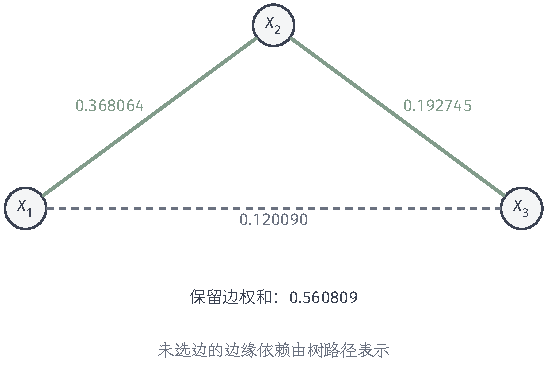
\includegraphics[width=92.650mm]{figures/09-probabilistic-graphical-models/03-learning/tikz/pgm-structure-learning-chow-liu/figure.pdf}
  \caption{计数表的互信息边权，单位为nat。最大权生成树保留实线两边，虚线是未选边。这个构造的经验分布恰好属于树族，因此可以精确复原；一般数据得到的是最佳树近似。}
  \label{fig:pgm-structure-learning-chow-liu}
\end{figure}

选$1$为根，根概率为$p(X_1=1)=0.5$，两条边的翻转概率为$0.1$、$0.2$。模型给出$\widehat p_{\mathcal{T}}(0,0,0)=0.5\times0.9\times0.8=0.36$；平均对数似然$-3\log2+0.368064+0.192745=-1.518633$，与前面评分计算相符。

证明中的正单点边缘用于保证条件概率分母有定义。零计数时可限制到经验支持，对从未出现的配置任选归一化条件表，并以$0\log0=0$延伸似然。若引入平滑伪计数，比较目标就随之改变。一般离散树的自由参数总数为
\[
  \sum_i(r_i-1)+
  \sum_{\{i,j\}\in E_{\mathcal{T}}}(r_i-1)(r_j-1).
\]
节点状态数相同等条件下，各树才有同一参数维数。状态数不同也不影响Chow--Liu对树族似然的精确优化，但BIC需扣除随边变化的参数惩罚，边权应作相应调整。

树约束同时简化学习与推断，也排除了环和不可约高阶作用。总体分布超出树族时，算法仍只能返回最佳树近似；互信息差异小时，抽样波动可能改变所选边。零权边也可能仅用于连接全节点，允许森林并惩罚边数则可保留断开的部分。

\subsection{高斯图结构学习}
\label{sec:pgm-structure-learning-gaussian}

对连续变量，高斯分布给无向结构学习带来一个极其优美的对应关系：联合高斯密度由协方差矩阵$\bm\Sigma$决定，但其逆矩阵$\bm K=\bm\Sigma^{-1}$（称为精度矩阵）的元素直接编码条件独立——精度矩阵里$K_{i,j}=0$，恰好等价于“给定其余所有变量后$X_i$与$X_j$独立”。直观上，$K_{i,j}$衡量的是把所有其他变量的影响都扣除后，$i,j$之间残留的直接关联；这一项为零，说明两者的相关完全可以由其余变量解释，它们之间不必有边。于是“学高斯无向图结构”被转化为“估计一个稀疏的精度矩阵”，这正是稀疏化方法可以大显身手的地方。要特别注意别和协方差混淆：$\Sigma_{i,j}=0$表示的是（不给定任何变量时的）边缘独立，而$K_{i,j}=0$才是条件独立，两者说的不是一回事。连续变量的条件依赖在高斯情形也有简洁表示。取$\bm{X}\sim\mathcal{N}(\bm{\mu},\bm{\Sigma})$、$\bm{\Sigma}\succ0$，\term{精度矩阵}（precision matrix）$\bm{K}=\bm{\Sigma}^{-1}$的零元素满足
\[
  X_i\perp X_j\mid\bm{X}_{V\setminus\{i,j\}}
  \quad\Longleftrightarrow\quad K_{i,j}=0.
\]
协方差零表示高斯边缘独立，精度零表示给定其余变量后的独立，二者约束不同。离开高斯分布后，逆协方差一般也失去这项条件独立解释。

由样本计算$\widehat{\bm{\Sigma}}=n^{-1}\sum_r(\bm{x}_r-\overline{\bm{x}})(\bm{x}_r-\overline{\bm{x}})^{\top}$，高斯负对数似然去常数并缩放后成为$-\log\det\bm{K}+\operatorname{tr}(\widehat{\bm{\Sigma}}\bm{K})$。直接把样本协方差求逆得到的精度矩阵通常是稠密的：由于抽样波动，几乎每个元素都只是很小、却不恰好为零，于是对应的图会变成全连接，没有揭示出真正的结构。要让无关的$K_{i,j}$被精确压成零，可以在高斯似然上加一个促使稀疏的$\ell_1$惩罚，这就是图Lasso；它同时完成“拟合高斯分布”和“筛出直接相连的边”两件事。小样本协方差可能奇异，直接求逆通常也不给稀疏零模式。对各变量样本方差严格为正的情形，\term{图Lasso}（graphical lasso）取$\lambda>0$，用非对角稀疏惩罚估计正定精度矩阵：
\begin{equation}
  \widehat{\bm{K}}
  =\argmin_{\bm{K}\succ0}
    \left\{-\log\det\bm{K}
      +\operatorname{tr}(\widehat{\bm{\Sigma}}\bm{K})
      +\lambda\sum_{i\ne j}|K_{i,j}|\right\}.
  \label{eq:pgm-structure-learning-glasso}
\end{equation}
上述样本方差与正惩罚条件保证唯一的有限正定最优解。若取$\lambda=0$，则需$\widehat{\bm{\Sigma}}\succ0$，最优解为其逆矩阵；零样本方差的变量应先移除或另行建模。

惩罚跳过对角，同时计算两个对称非对角元；只对$i<j$求和的实现需要换算$\lambda$。正定约束保持合法密度，$\ell_1$项允许估计出现精确零。目标是凸函数，可以用凸优化方法求解，抽样误差及选边正确性仍需统计条件\scite{pgm-structure-learning-friedman2008}

还可从每个节点的条件预测选择邻居。高斯条件均值为
\[
  \mathbb{E}[X_i\mid\bm{X}_{-i}]
  =\mu_i+\sum_{j\ne i}
    \left(-\frac{K_{i,j}}{K_{i,i}}\right)(X_j-\mu_j),
\]
$-i$表示其余全部节点，回归系数的非零模式因而对应邻居。分别作稀疏回归后，两端可能对同一边作不同选择；OR取并集，较多保留边，AND取交集，较少保留边。联合密度还需对称正定的精度矩阵，因此各节点独立回归后应继续检查或拟合相容参数。

例如取以下精度与协方差：
\[
  \bm{K}=
  \begin{pmatrix}
    2&-1&0\\
    -1&2&-1\\
    0&-1&2
  \end{pmatrix},
  \qquad
  \bm{\Sigma}=\frac14
  \begin{pmatrix}
    3&2&1\\
    2&4&2\\
    1&2&3
  \end{pmatrix}.
\]
两矩阵相乘为单位阵，精度矩阵顺序主子式为$2,3,4$，故正定。$\Sigma_{1,3}=1/4$显示边缘相关，$K_{1,3}=0$则说明给定$X_2$后独立。节点$1$仅回归到$X_2$，系数$1/2$；节点$2$对两端的系数也均为$1/2$，得到同一链。实际调参应按用途评价$\lambda$，预测误差最小与精确选边可能需要不同取值。

\subsection{离散与高阶Markov网络结构学习}
\label{sec:pgm-structure-learning-discrete}

树和高斯特例之所以好算，是因为只需要决定成对的边；但一般离散分布里，变量之间可能存在“三个变量才一起出现、任何两个单独看都独立”的高阶相互作用，这种结构无论怎么连成对边都表达不出来。因此一般离散无向模型的结构学习必须直接选择作用在任意变量子集上的特征（团），候选数量与归一化成本都随之上升。一般离散分布需要直接选择相互作用。先规定特征字典$\{f_a(\bm{x}_{C_a})\}$，$C_a\subseteq V$表示每个特征涉及的节点，再用有限状态的正指数模型表示概率：
\[
  p_{\bm{\theta}}(\bm{x})
  =\exp\!\left\{\sum_a\theta_a f_a(\bm{x}_{C_a})
                    -A(\bm{\theta})\right\}.
\]
参数的非零模式决定哪些相互作用参与模型。同一作用域有多项编码时，可用组稀疏惩罚共同选取；编码需可识别或有对比约束，使零系数具有确定含义。高阶因子的作用域在无向图中成为团，因此因子集合还能区分同一边图中的不同高阶关系。

用$\widehat{\mathbb{E}}[f_a]$表示经验特征均值，取$\lambda>0$并惩罚全部参数，完整似然的稀疏估计为
\[
  \min_{\bm{\theta}}\left\{
    A(\bm{\theta})-\sum_a\theta_a\widehat{\mathbb{E}}[f_a]
      +\lambda\lVert\bm{\theta}\rVert_1\right\}.
\]
正惩罚使参数趋于无穷时目标发散，从而存在有限最优参数。取$\lambda=0$时，需另查无罚最大似然估计是否存在；某些经验零频率会使目标仅在参数趋于无穷时逼近下确界。

梯度含模型期望，每轮都要进行推断；大团或大树宽会反复增加这项成本。\term{伪似然}（pseudolikelihood）改用各节点条件概率的乘积$\prod_{r,i}p_{\bm{\theta}}(x_{r,i}\mid\bm{x}_{r,-i})$。它只在单节点状态上归一化，可绕过全局配分函数；评价其统计效率与有限样本性质时，需要针对这个替代目标分析。

在成对Ising模型中，取$x_i\in\{-1,1\}$，局部场$u_i=b_i+\sum_{j\ne i}J_{i,j}x_j$汇总其他节点的作用。单点条件对数赔率为
\[
  \log\frac{p(X_i=1\mid\bm{x}_{-i})}
                {p(X_i=-1\mid\bm{x}_{-i})}=2u_i.
\]
该对数赔率使邻域估计化为稀疏逻辑回归。共同优化对称参数$J_{i,j}=J_{j,i}$时，条件概率来自同一联合模型；逐节点分别拟合时，还要协调两端选边与参数。直接搜索因子也可使用精确、近似或伪似然评分，应明确实际比较的目标。

成对边缘还可能隐藏高阶关系。以下正分布给出一个三变量反例：
\[
  p(x_1,x_2,x_3)
  =\frac{\exp(\theta x_1x_2x_3)}{8\cosh\theta},
  \qquad x_i\in\{-1,1\},\quad \theta\ne0.
\]
消去任一变量，分子变为$2\cosh\theta$，每对边缘都是$1/4$，故成对互信息为零。三阶矩却满足$\mathbb{E}[X_1X_2X_3]=\tanh\theta\ne0$，给定$X_3$后两端仍有相互作用。这个处处正的分布需要三阶特征，说明成对独立不足以推出联合独立。若允许大小至多$m$的作用域，候选子集数为$\sum_{\ell=1}^{m}\binom d\ell$，每个离散作用域还可能有多个参数，搜索及样本成本随之增长。

\subsection{潜变量结构的学习}
\label{sec:pgm-structure-learning-latent}

到此为止都假设数据里的变量就是全部相关变量。但现实中观测到的一大堆变量可能只是少数几个\emph{未观测共同原因}的结果——例如若干传感器读数相关，仅仅因为它们都受同一个隐藏的环境温度驱动。若不知道这个隐变量、直接在观测变量间学图，就会在本无直接关系的变量之间连出稠密的一团边。结构学习因此还要区分：哪些依赖在把隐变量考虑进来后仍真实存在，哪些依赖只是共同隐变量投下的“影子”。稠密观测关系还可能由共同隐变量产生。此时直接恢复观测边缘图，会把共同隐变量造成的关系与观测变量之间的条件关系混在一起。结构学习需要进一步判断：哪些依赖在给定潜变量后仍然保留，哪些依赖可以由少量共同潜在方向解释。将联合高斯节点分为观测集合$O$和潜变量集合$H$，按两组分块精度矩阵。积分潜变量或对二次型配方后，观测边缘的精度为
\begin{equation}
  \begin{aligned}
    \bm{K}_{\mathrm{marg}}
      &=(\bm{\Sigma}_{O,O})^{-1}\\
      &=\bm{K}_{O,O}
        -\bm{K}_{O,H}\bm{K}_{H,H}^{-1}\bm{K}_{H,O}\\
      &=\bm{S}-\bm{L}.
  \end{aligned}
  \label{eq:pgm-structure-learning-schur}
\end{equation}
$\bm{S}=\bm{K}_{O,O}$表示给定潜变量后的条件精度；$\bm{L}\succeq0$且秩至多$|H|$表示边缘化带来的修正。条件图稀疏、有效潜变量少时，这构成常称的\term{稀疏加低秩分解}（sparse plus low-rank decomposition）。名称强调两种结构，按此处半正定约定实际以减法组合。

取$X_i=Z+\varepsilon_i$，$i=1,2,3$，并令$Z,\varepsilon_1,\varepsilon_2,\varepsilon_3$相互独立且均为标准高斯。给定$Z$后三个观测独立；积分$Z$后协方差为$\bm{I}+\bm{1}\bm{1}^{\top}$，其逆可直接验证为
\[
  \bm{K}_{\mathrm{marg}}
  =\bm{I}-\frac14\bm{1}\bm{1}^{\top}.
\]
所有非对角元为$-1/4$，所以观测条件图完整，而$\bm{S}=\bm{I}$、$\bm{L}=\bm{1}\bm{1}^{\top}/4$只有一个潜在修正方向。边缘依赖与给定共同潜变量后的独立，描述的是不同条件分布。

根据观测样本协方差$\widehat{\bm{\Sigma}}_{O,O}$，取$\lambda>0$，可以同时拟合这两种结构：
\begin{equation}
  \begin{aligned}
    \min_{\bm{S},\bm{L}}\quad&
      -\log\det(\bm{S}-\bm{L})
      +\operatorname{tr}\!\left(
           \widehat{\bm{\Sigma}}_{O,O}(\bm{S}-\bm{L})\right)\\
      &+\lambda\bigl(\gamma\lVert\bm{S}\rVert_1
                      +\operatorname{tr}(\bm{L})\bigr),\\
    \text{满足}\quad&\bm{S}-\bm{L}\succ0,\qquad \bm{L}\succeq0.
  \end{aligned}
  \label{eq:pgm-structure-learning-sparse-low-rank}
\end{equation}
$\lVert\bm{S}\rVert_1$逐元素求绝对值，包含对角；$\gamma>0$调节稀疏与低秩惩罚的相对强度。正惩罚控制精度矩阵及潜变量修正的增长，使有限正定最优解存在。取$\lambda=0$时，仍需观测样本协方差正定，边缘精度的最优解才是其逆矩阵，$\bm S$与$\bm L$的分解则可能不唯一。

半正定矩阵的核范数等于迹，所以第二项鼓励低秩。该凸程序的恢复保证还需两类结构足够可区分，例如潜变量作用分散于较多观测节点，避免低秩项本身也高度稀疏\scite{pgm-structure-learning-chandrasekaran2012}

若某分量同时稀疏、低秩，它可以在两项间移动而不改变差，精确边缘精度也可能无法确定唯一分解。满足识别条件时，$\bm{L}$的秩表示有效潜在维数，潜变量的物理个数、旋转与含义仍需额外信息。完整潜变量图、条件图$\bm{S}$和边缘观测图$\bm{K}_{\mathrm{marg}}$因此应分别解释；低秩分解回答统计结构问题，尚未识别潜在因果机制。

\section{因果发现}
\label{sec:pgm-structure-learning-causal}

本章前几节学到的图，严格说只表示变量在\emph{被动观测}下的联合分布；而等价类的存在意味着，光凭这种分布往往无法确定箭头方向。但在很多决策问题里我们真正想问的是“如果人为去改变某个变量会怎样”——降低温度会不会真的减少故障？这是一个\emph{干预}问题，需要把箭头读作因果机制。本节就讨论：在观测数据基础上，需要补上哪些假设或哪类实验数据，才能把结构（哪怕部分地）解释为因果结构。到这里，图用于表示联合分布。若要预测外部改变某变量的后果，还需给局部关系赋予干预含义。接下来比较不同信息与假设能识别到什么结构，让输出对应可以成立的因果结论。

\subsection{因果假设与识别目标}
\label{sec:pgm-structure-learning-causal-assumptions}

要把观测到的图当因果图用，必须先明确几条无法仅靠数据证明、需要由问题背景背书的假设。最核心的是因果Markov性与忠实性这一对：前者保证“因果结构会产生我们能观测到的独立约束”，后者保证“观测到的独立都能归因于结构”，两者合起来才允许从独立性反推因果方向。因果Markov性要求每个变量在给定其直接原因后，与非后代独立；忠实性则要求分布中的条件独立都由图上的d-分离解释。前者从机制导出独立约束，后者支持从独立关系反推图，但观测等价仍会限制方向识别（参见\BookChapterRef{chap:causal-inference}{卷2《数学准备：概率、因果与决策》的“因果响应”章}）。本节在这些条件下考察可识别输出，再说明潜在混杂、函数形式及干预如何提供不同信息。

当前变量是否覆盖共同原因，也影响图的解释。\term{因果充分性}（causal sufficiency）要求它们的共同原因都已观测，即当前模型没有遗漏潜在混杂。它只针对所选节点集合，通常还需无环过程、已声明的数据环境及适当处理选择偏差。以函数形式识别更多方向时，还要加入相应线性、噪声独立或非高斯条件；搜索方法使用这些假设，却不能自行验证它们成立。

因果充分、无环且忠实时，观测独立信息一般确定CPDAG。一旦允许存在未观测的共同原因，CPDAG就不够用了：它无法表达“两个观测变量的相关其实来自一个潜混杂”这种关系，而把隐变量显式画出来又会让图无限膨胀、且我们根本不知道有几个隐变量。需要一种只画观测变量、却能用不同端点记号同时表达“祖先方向”和“由潜变量造成的混杂”的图。允许潜变量后，需表示边缘化留下的关系。\term{最大祖先图}（maximal ancestral graph, MAG）用有向、双向及处理选择偏差时的无向边表达观测独立性，省去潜变量的显式细节。合法图无有向环；箭头端不能是另一端的祖先，无向边的端点不能再接指入箭头。“最大”表示每对不相邻节点都能由某组观测量分离。对应的\term{m-分离}（m-separation）按两侧箭头辨认路径碰撞点：活跃路径要求非碰撞点不在条件集中，每个碰撞点自身或某个后代在条件集中；两端没有活跃路径时才被分离。

多张MAG也可能具有相同独立关系，\term{部分祖先图}（partial ancestral graph, PAG）保留这类图共同的端点信息。尾端和箭头端为类内不变标记，圆圈表示端点尚未确定，边本身仍存在。无选择偏差时，$i\to j$表示祖先关系，$i\leftrightarrow j$排除互为祖先且与潜在混杂相容，$i\mathbin{\circ\!\!\to}j$只确定$j$端箭头。这些标记表达祖先与独立性的不确定性，未给出直接因果机制、双向反馈或潜变量的具体个数和连接\scite{pgm-structure-learning-zhang2008}

\subsection{基于观测数据的因果发现}
\label{sec:pgm-structure-learning-observational}

先看在不做实验、只有观测数据时，靠不同强度的假设最多能把方向确定到什么程度：最基本的PC/GES只能给CPDAG；允许潜在混杂的FCI给更保守的PAG；而借助“线性+非高斯噪声”等函数形状假设，LiNGAM、ANM等方法有时能打破观测等价、唯一确定方向——代价是假设强得多。PC与GES得到的统计等价类，要在因果假设下才能解释为因果等价类（参见第~\ref{sec:pgm-structure-learning-directed}节）。PC在因果Markov性、忠实性、充分性、无环性及准确独立判定下返回CPDAG，有限样本返回其估计。GES则需要评分等价、可分解且局部一致，真实分布忠实于候选有向图，并满足固定维大样本条件。这里局部一致性具体指：样本足够多时，评分奖励补上遗漏依赖，惩罚多余依赖；在这些条件下等价类搜索可恢复CPDAG。

潜在混杂会改变需要检查的分离集合。\term{快速因果推断算法}（fast causal inference, FCI）扩展PC的搜索范围并采用祖先图定向规则，在相应Markov性、忠实性和准确独立信息下输出PAG。标准框架还可处理声明的选择机制。无限观测数据也可能只确定这个部分对象，圆圈应继续保留；完整规则及识别范围见Zhang的研究\scite{pgm-structure-learning-zhang2008-completeness}

分布形状可以提供独立关系之外的方向信息。\term{线性非高斯无环模型}（linear non-Gaussian acyclic model, LiNGAM）以独立扰动驱动各节点：
\[
  X_j=\sum_{i\in\operatorname{pa}(j)}b_{j,i}X_i+\varepsilon_j,
\]
图取无环，扰动相互独立、非高斯且方差有限非零，并排除未观测混杂。令$B_{j,i}=b_{j,i}$，递归方程给出$\bm{X}=(\bm{I}-\bm{B})^{-1}\bm{\varepsilon}$。这里用到的\term{独立成分分析}（independent component analysis, ICA）本是一种信号分离技术（经典例子是把多个麦克风录到的混合人声按“各声源相互独立”还原出来）；在LiNGAM中它被借来从观测变量的混合中分离出相互独立的非高斯扰动；非高斯性用来区分各个扰动来源，无环约束再用来解决“分离出的分量该对应到哪个变量”的排列歧义，于是可在模型条件下识别超出MEC的方向。线性高斯分布缺少这种方向信息，识别结论依赖所保留的非高斯条件\scite{pgm-structure-learning-shimizu2006}

非线性函数也可能使方向不对称。\term{加性噪声模型}（additive noise model, ANM）取$Y=f(X)+\varepsilon$、$\varepsilon\perp X$；在满足相应光滑性、非退化和可识别性条件的模型中，反向无法同时写成$X=g(Y)+\eta$、$\eta\perp Y$。因此可比较输入与拟合残差的独立性，而不只比较回归误差。多变量形式还需递归机制及独立扰动；线性高斯等双向可表示情形属于识别例外\scite{pgm-structure-learning-peters2014}

\subsection{基于干预数据的因果发现}
\label{sec:pgm-structure-learning-interventional}

既然纯观测数据困在等价类里，打破僵局最直接的办法就是做实验：主动去\emph{设置}（干预）某个变量的值，而不只是观察它。干预会切断该变量与其自然原因之间的联系，从而制造出观测数据中不存在的不对称——三张观测等价的图，在同一个干预下往往给出明显不同的预测。观测和干预的差别可以继续用计数表说明。观测$X_2=1$时，$X_1=1$的频率为$0.9$；外部设置$X_2$却改变了数据产生方式。正向链$X_1\to X_2\to X_3$中，改变中间变量不影响其上游$X_1$；分叉$X_1\leftarrow X_2\to X_3$中，$X_1$随之改变。这类实验能区分相同被动观测支持的机制。

为计算这种改变，\term{完美干预}（perfect intervention）替换目标节点的机制、切断它对原父节点的依赖，同时保持其他机制。取已知目标集合$I\subseteq V$，各目标独立随机化并使用外部规定的$q_i^I$，干预分布为
\begin{equation}
  p^I(\bm{x})
  =\prod_{i\in I}q_i^I(x_i)
   \prod_{j\notin I}
      p(x_j\mid\bm{x}_{\operatorname{pa}_{\mathcal{G}}(j)}).
  \label{eq:pgm-structure-learning-intervention}
\end{equation}
图上删去进入$I$的全部箭头，得到$\mathcal{G}^{[I]}$；$I=\varnothing$给回观测环境。固定目标值可作为退化干预。以独立信息刻画等价类时，需要足够支持的随机化或覆盖相关取值的实验，以免变量固定造成额外退化。

记目标集合族为$\mathcal{I}$。若每个节点至少在一个环境未受干预，该族称为\term{保守的}（conservative），包含观测环境即满足。给定目标及完美干预规则后，允许相同多环境分布族的有向无环图构成\term{干预Markov等价类}（interventional Markov equivalence class, I-MEC）。各环境共享非目标机制，因而这里比较的是协调的多环境模型。

在保守目标族及相应正性条件下，两图干预等价恰好要求观测Markov等价，并且每个$I\in\mathcal{I}$下的删入边图具有相同骨架。也可用观测骨架与v-结构相同，再比较各干预图的Markov等价关系来刻画。\term{干预本质图}（interventional essential graph）把I-MEC共同方向画成箭头，其余边保持无向。干预细分了观测MEC，但目标不足时仍可能保留多张候选图\scite{pgm-structure-learning-hauser2012}

将三种观测等价图都拟合到同一二值表，再作$\operatorname{do}(X_2=1)$。正向链预测$(p(X_1=1),p(X_3=1))=(0.5,0.8)$，分叉为$(0.9,0.8)$，反向链为$(0.9,0.5)$；仅观测$X_2=1$时，三者却都给$(0.9,0.8)$。图~\ref{fig:pgm-structure-learning-intervention}展示这组差异：在给定总体假设下，覆盖$X_2$两种取值的完美干预足以区分它们。有限实验还需评价频率估计误差。

\begin{figure}[!t]
  \centering
  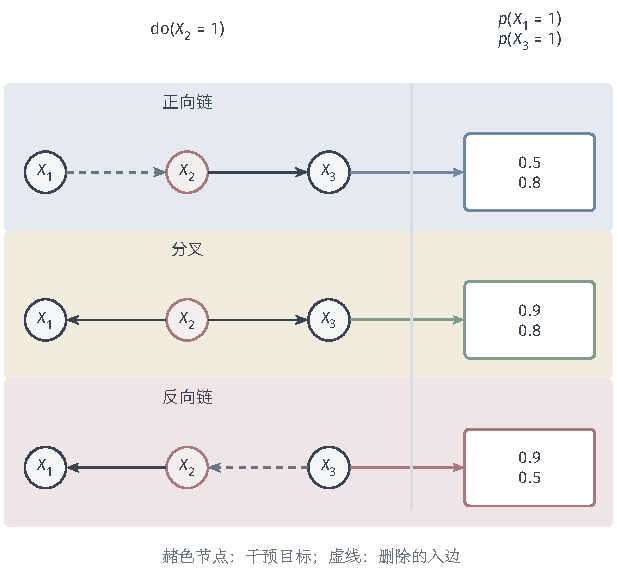
\includegraphics[width=104.405mm]{figures/09-probabilistic-graphical-models/03-learning/tikz/pgm-structure-learning-intervention/figure.pdf}
  \caption{干预$X_2$对同一观测MEC的三种预测。蓝、黄、红横带依次为正向链、分叉、反向链，右侧概率框及连接箭头对应各结构的预测。实线保留非目标机制，虚线表示切断的入边；在给定三节点设定下，预测差异提供方向信息。}
  \label{fig:pgm-structure-learning-intervention}
\end{figure}

\term{贪心干预等价搜索}（greedy interventional equivalence search, GIES）直接在干预本质图空间比较I-MEC，采用前向、后向及转向操作。每条记录需带目标标签$I_r$；目标随机化分布已知或独立于候选图时，去掉共同常数后的机制对数似然为
\[
  \ell(\mathcal{G},\bm{\theta})
  =\sum_{r=1}^{n}\sum_{j\notin I_r}
       \log p_{\bm{\theta}_j}
          (x_{r,j}\mid\bm{x}_{r,\operatorname{pa}(j)}).
\]
目标节点的观测不用于拟合它的原机制，仍可进入子节点的机制拟合。各机制可用样本数不同，惩罚评分需要体现这种多环境设定。GIES据此汇合观测与干预证据；具体搜索最优性及因果恢复仍须结合评分、样本和模型条件分析。

未知目标时，环境标签只说明有机制变化，还需限定哪些机制可变、变化是否可检测及其余机制如何保持，再联合推断目标。软干预只改机制的一部分而保留父依赖，也需要修改删边表示和I-MEC定义。执行不依从、目标不完全、非目标机制漂移或潜在混杂都会改变识别范围，应使用与这些条件相容的模型。

已有候选还可用于决定下一次实验。\term{主动实验设计}（active experimental design）在可执行且满足预算的目标中，选择预计最能区分候选的干预；三节点例子的中间节点就是一项选择。预期后验熵下降、待定端点减少或科学查询的区分度都可作为准则，并需计入成本。这些预期仍依赖当前模型和机制不变假设，实验实施后的证据要另外评价。

表~\ref{tab:pgm-structure-learning-causal-routes}把信息、假设和输出放在同一口径下比较。路线可以交叉：ANM可使用回归及独立检验，连续优化也可处理特定函数模型。识别能力由数据和模型条件决定，求解工具规定如何利用这些信息。

\begin{table*}[htbp]
  \centering
  \small
  \begin{tabularx}{\linewidth}{@{}lXX@{}}
    \toprule
    路线 & 关键条件与信息 & 理想识别对象及限制 \\
    \midrule
    PC & 无环、因果充分、Markov且忠实；准确独立性信息 & CPDAG；不决定类内可逆方向 \\
    GES & 相应充分有向图模型；评分等价、可分解、局部一致 & 大样本下CPDAG；不是一般贪心搜索的保证 \\
    FCI & 允许潜在混杂；相应Markov性、忠实性及选择机制假设 & PAG；不是潜变量完整图 \\
    LiNGAM & 线性无环、独立非高斯扰动、无潜在混杂 & 模型条件下单个有向图；依赖分布形状 \\
    ANM & 独立加性噪声、无混杂及特定可识别性条件 & 满足条件时单个有向图；存在双向可表示例外 \\
    GIES & 已知目标的完美干预、无混杂、机制不变、相应评分 & 搜索I-MEC；并非一般全局最优保证 \\
    \bottomrule
  \end{tabularx}
  \caption{不同假设下的识别目标。表列理想输出以总体条件成立为前提；实际估计还包含抽样、拟合与搜索误差，因此需同时说明假设和计算过程。}
  \label{tab:pgm-structure-learning-causal-routes}
\end{table*}

\subsection{因果发现的边界}
\label{sec:pgm-structure-learning-causal-limits}

因果发现的结论有多可信，必须把“不确定”按来源分清楚，因为三种不确定性的补救办法完全不同：样本太少带来的统计误差靠补数据解决；假设错了会让更多数据反而更坚定地指向错误的图；而总体层面的不可识别则再多数据也无用、只能靠新假设或新实验。不确定性需要按来源判断。样本误差使检验和评分偏离总体结果，增加同类记录有机会降低它。假设错误可能让更多数据稳定地支持错误图，例如有混杂却使用充分性模型。总体不可识别则意味着多个候选在所有允许资料下都产生同一分布，需要增加信息才能区分。这三种情况分别指向补样本、改模型及设计实验。

等价类中的未定向边和PAG圆圈保留的是资料尚未确定的信息。领域知识可以排除候选，应标明它贡献的方向；函数形式可以缩小等价范围，也需核验对应假设。稀疏、有向且重复得到的图仍只说明特定流程的结果，因果解释需要这些额外依据。

结构发现之后，干预效应是否可计算仍是另一项识别问题，do演算和反事实查询有各自定义及条件。本节得到的部分结构为这些查询提供约束，具体效应和个体反事实还需按对应问题分析。

\section{算法分析}
\label{sec:pgm-structure-learning-analysis}

参数学习的评价相对直接（估计值离真值多近、预测准不准），结构学习的评价却更微妙：算法可能恢复错了方向却恰好预测得不错，也可能在有限样本上不稳定，还可能因为算不动而只找到局部最优。系统地评价一种结构学习方法，要分别回答三个不同层面的问题。评价结构学习可以沿三个问题展开：候选图及局部函数能表示哪些分布；搜索能否找到目标候选、以多少计算完成；有限样本下选出的结构与预测能否接近总体目标。下面分别检查统计一致性、计算成本和评价协议，使“最优”“一致”与“稳定”各有明确对象。

\subsection{统计一致性与有限样本误差}
\label{sec:pgm-structure-learning-consistency}

首先要区分“估计得准不准”和“问题本身能不能确定”。结构学习的一致性必须针对一个\emph{可识别的目标}来谈——当观测数据只能确定CPDAG时，要求算法稳定地恢复出某一张特定方向的有向图本身就不合理，正确目标应是那个等价类。先把可识别目标记为$\mathcal{C}^{*}$，例如CPDAG；\term{结构一致性}（structural consistency）要求$\mathbb{P}(\widehat{\mathcal{C}}_n=\mathcal{C}^{*})\to1$。目标必须与可用信息匹配。真实分布超出树族时，Chow--Liu可以趋向最佳树近似；图Lasso参数误差趋零时，精确零模式还需非零信号与零之间有足够间隔。

PC需要全部相关独立判定同时正确。若检验集合大小为$M$、每项错误概率至多$\delta$，联合界给出至少一项检验出错的概率至多$M\delta$，无需检验独立。自适应选择时应覆盖全部可能用到的检验，而非事后只数执行次数。若要整体错误随$n$消失，固定显著性水平通常不足，还需合适阈值序列及功效条件。

最弱依赖往往决定可恢复程度。高斯偏相关小于估计波动时难以检出；离散条件集扩大后，每个配置的记录更少。稀疏图有助于限制条件集，同时仍需控制最大度、状态数、协方差条件数或最小信号，才能给出具体一致性结论。

BIC比较也依赖固定维、正确模型和正则条件。遗漏依赖通常带来随$n$线性增长的似然损失，多余参数的随机拟合收益通常仅为有界概率量级，$\log n$惩罚据此区分两者。这个理由说明评分的候选比较；搜索若未到达相关模型，还需另外控制搜索误差。潜变量奇异或维数增长时，应重查渐近尺度。

树的稳定性可以由边权间隔直接说明。取$d\geq3$且总体最大权生成树唯一，对非树边$e$与其连接路径上的树边$f$，定义
\[
  \Delta=\min_{e\notin E_{\mathcal{T}^{*}}}
             \min_{f\in\operatorname{path}_{\mathcal{T}^{*}}(e)}
             \{I_f-I_e\}.
\]
若$\Delta>0$且所有互信息估计误差小于$\Delta/2$，非树边与路径边的次序保持，最大权树也保持。教学例子中间隔约为$0.072654$，等于较小两条互信息的差。零间隔可能容许多棵最优树，分布预测相近时具体选边仍可能变化。

\subsection{计算复杂度与可扩展性}
\label{sec:pgm-structure-learning-complexity}

一致性回答“样本足够多时能否恢复对的结构”，但实践中还要问“要花多少计算、规模一大还算不算得动”。结构学习的开销主要来自在巨大图空间里反复做检验或评分，下面按主要算法分别给出规模量级。计算成本要按实际搜索规模估计。PC枚举条件集并逐项检验；整个过程中候选邻域至多$q$时，粗略检验数为$O(d^2 2^q)$，总时间还乘单次检验成本。误保留边会增大候选邻域，故$q$未必等于真实最大度。FCI扩大了分离集搜索范围，也增加相应运算。

离散有向图可缓存局部评分，候选父集数量仍可能指数增长。预计算最佳父集表后，常见动态规划递推约需$O(d2^d)$时间，表的准备及内存另计；整数规划的分支搜索同样可能指数增长。局部搜索每轮约检查$O(d^2)$个移动，总成本还取决于轮数、无环检查及拟合，需与单轮操作数分开。

状态数有界时，Chow--Liu以$O(nd^2)$时间汇总成对计数，再以稠密Prim的$O(d^2)$或排序Kruskal的$O(d^2\log d)$求树。固定树上的有限状态边缘推断随节点数线性增长。这两项计算收益来自树约束，也伴随其表示能力限制。

稠密NOTEARS每次残差乘法约需$O(nd^2)$，矩阵指数通常需$O(d^3)$规模的线性代数，总时间还乘内部优化及惩罚更新轮数。图Lasso有矩阵更新成本，凸性则方便检查求解误差；逐节点回归易并行，联合参数相容性需继续处理。高阶离散评分还可能反复计算配分函数。限制父集或作用域时，应说明节省的计算和排除的候选。

\subsection{结构评价与稳定性}
\label{sec:pgm-structure-learning-evaluation}

有了已知真值的仿真数据，就能直接量化“学出的图和真图差多远”，但要注意骨架对错与方向对错应分开计分，并且当目标本就是等价类时，不应因为可逆方向没猜中而扣分。仿真有已知生成结构时，可分别测量骨架与方向。骨架精确率为正确边数除以预测边数，召回率为正确边数除以真实边数，零分母规则需预设。方向评价需说明是否计入漏边。若资料只能识别CPDAG，应以该类为目标，既不因未选中某代表的可逆方向罚分，也不把偶然猜中当作识别收益。

最常用的单一指标是直接数“要把学出的图改成真图，至少做多少次边的增删改”。\term{结构Hamming距离}（structural Hamming distance, SHD）就计量估计图变到目标图所需的边编辑数，数值为零表示两图完全一致；常见约定将加边、删边、反向各计1，也有把反向计为删加两步的实现，比较时需固定口径。CPDAG评价先将生成有向图转为等价类，再比较邻接、被迫方向和未定向状态；PAG还需比较圆圈、尾端及箭头端。

真实数据通常没有一张“真图”可供对照打分。退而求其次的办法是考察结果的\emph{稳定性}：若换一批略有不同的样本，学出的图就面目全非，说明这些边并不可靠；若某些边在各种扰动下都反复出现，则更可信。实现这种扰动的标准手段是对原数据有放回地重复抽样。真实记录缺少标准答案时，可测量结果对重采样的敏感性。\term{自助重采样}（bootstrap）从$n$条独立记录有放回抽$n$条，重复拟合$B$次，将边出现频率写为
\[
  \widehat\pi_{i,j}
  =\frac1B\sum_{b=1}^{B}
       \mathbf{1}\{\{i,j\}\text{在第}b\text{次结果中相邻}\}.
\]
方向需另计频率，并声明分母取全部重复还是该边出现的重复。CPDAG未定向边应保留该状态；各轮是否重做筛选与调参，也影响所测流程。多环境资料在环境内重采样，相关序列则按适当块抽样，使评价单位符合数据依赖。

重采样频率表示流程对数据扰动的敏感性；错误先验或模型假设也可能产生稳定结果，因此它不同于结构后验及因果真实性概率。还可比较合理正则、检验和模型设置，并在未参与选图与调参的记录上报告平均预测对数概率或对数密度，值越大表示给真实观测的预测支持越高。这项预测评价仍未验证因果方向。

领域知识也可明确限制候选。禁止$i\to j$就排除$X_j$父集中含$X_i$的选项，必选$i\to j$则保留包含$X_i$的父集；时间顺序排除逆时间箭头。搜索前需检查约束相容且无环；等价类结果还应区分数据确定与知识补充的方向，并相对于加入同一知识后的识别目标评价。

\section{本章小结}
\label{sec:pgm-structure-learning-summary}

从记录到图，需要分别判断局部独立证据、整体模型得分和合法空间搜索。检验说明哪些联系可由给定变量隔断，评分权衡拟合与复杂度，搜索组织候选比较。树之所以可精确求解，是因为最优似然化为互信息边权和；一般有向图和高阶无向模型还要承担更大的搜索或归一化成本。

同一张计数表可支持无向链、观测等价类及结构后验，却不能仅由频率选定因果方向。缺失观测引入后验统计量，潜变量边缘化可能使稀疏条件图变稠密；改变的不只是运算，也包括可识别对象。赋予结构因果解释时，需明确机制、混杂、忠实性和函数形式假设，才能判断结果是CPDAG、PAG还是干预等价类中的信息。

回到设备记录，数据能够帮助选择依赖表示，故障传播方向还需相应识别条件和干预依据。增加同类样本可以在相应统计条件下降低估计误差；改善搜索用于控制优化误差，修改假设用于处理模型偏差，总体观测等价则可能仍需新实验。因此报告结构时，应同时给候选范围、数据与干预条件、检验或评分、搜索限制及保留的不确定性。

接下来的模型以具体任务选择这些结构：分类、潜在分组和状态估计各有其表达与计算要求。静态有向模型把局部分解、推断和学习用于此类任务（参见第~\ref{chap:pgm-static-directed}章）。结构适合计算和预测时，潜变量的物理含义仍可能需要其他证据。

\paragraph{扩展阅读}
Koller与Friedman的教材进一步展开条件独立检验与评分搜索，可按本章的计数、等价类和搜索目标继续阅读。理解统计分解之后，再核对因果解释增加了哪些机制与识别条件\scite{pgm-koller2009}

